\documentclass[10pt]{article}

\usepackage{titlesec}
\usepackage[singlespacing]{setspace}
\usepackage[letterpaper,margin=0.75in]{geometry}

\setcounter{tocdepth}{4}


\usepackage{hyperref}
\usepackage{geometry}
\usepackage{graphicx}
\usepackage{float}

\usepackage{lastpage}
\usepackage{fancyhdr}
\fancyfoot[C]{Page \thepage\ of \pageref{LastPage}}

\usepackage{listings}
\usepackage{color}

\definecolor{codegreen}{rgb}{0,0.6,0}
\definecolor{codegray}{rgb}{0.5,0.5,0.5}
\definecolor{codepurple}{rgb}{0.58,0,0.82}
\definecolor{backcolour}{rgb}{0.95,0.95,0.92}

\lstdefinestyle{mystyle}{
    backgroundcolor=\color{backcolour},
    commentstyle=\color{codegreen},
    keywordstyle=\color{magenta},
    numberstyle=\tiny\color{codegray},
    stringstyle=\color{codepurple},
    basicstyle=\footnotesize,
    breakatwhitespace=false,
    breaklines=true,
    captionpos=b,
    keepspaces=true,
    numbers=left,
    numbersep=5pt,
    showspaces=false,
    showstringspaces=false,
    showtabs=false,
    tabsize=2
}

\lstset{style=mystyle}

\begin{document}
\pagenumbering{gobble}
\begin{titlepage}
    \title{Project Hand Off}
    \author{Yeongae Lee, Jaehyung You \\ CS 463  \\ Oregon State University \\ Spring 2019 \\ \\ Project Physics Virtual Classroom: AsyncSync (Group 51) \\by Physics Department \\Dr. Kenneth Walsh}
    \date {June 10, 2019}


    \maketitle
        \begin{abstract}
            The project Physics Virtual Classroom, which is suggested by Physics department at Oregon State University, aims to build the web page which students can take online lectures. The distinctive difference between this website and other online lecture websites is that it uses live lectures to engage students. With live lectures, students can ask questions and professors can answer questions. In addition, by setting up group activities in the middle of the class, students will be able to develop their ability to solve problems through collaboration. This document describes the requirements for building this website. The ultimate goal of the project is to allow that students can work together and have a better educational environment.
            This document includes all the work we have done for a year. The documents are requirement documents, design documents, tech reviews, Weekly Blogs posts, final poster, project documentation, useful resources, and our reflections.




        \end{abstract}
\end{titlepage}
\newpage
\pagenumbering{arabic}

\tableofcontents
\newpage

\section{Introduction}
    This project is suggested by Dr. Kenneth at Oregon State University in the Physics Department. He graduated from Oregon State University with a Bachelor of Science in Physics and Engineering Physics. He remained at Oregon State University to complete his Doctorate of Philosophy in physics. He wants OSU students to improve their understanding of the material by collaborating on problems, instead of working alone. Students can improve their problem-solving skills by freely exchanging and sharing ideas on the whiteboard. Live lectures encourage active participation of students by allowing students to ask questions in real time. Students experience a better learning environment because of the increased accessibility of educational tools. Team AsyncSync worked on this project. Yeong-ae Lee worked on adding lecture video and designing main lobby page. Jaehyung You focused on implementing whiteboards and the cheat system. Client and head programmer supervised the project. The client envisioned an outline of the overall project. The head programmer provided ideas for technical parts which are the development environment and server. This change in the educational paradigm will be an important beginning for not only studying in physics, but it also helps to improve the efficiency and the quality of all studying in the future.

\section{Requirements Document}
    \subsection{Introduction}
        \subsubsection{System Purpose}
            The system is designed to provide online lectures which can communicate with instructors in real time to introductory physics students at Oregon State University(OSU). It is an open source learning platform. The system will allow instructors and professors to continuously adapt learning materials to facilitate the online learning experience for students. Furthermore, another goal is generating data about the learning tools being used, which will allow researchers to study the efficacy of the learning material and the system. Lastly, the system is meant to increase communication, and dialogue between students while learning. This system will give students the option to work on problems simultaneously, share ideas and help one another learn.

        \subsubsection{System Scope}
            Our objective is to create a website for Physics students. The website will have features that include the live-session page, where students will take a live lecture, and online-interactive shared whiteboard, which will allow students to collaborate on homework in real-time. It will provide an area in which they can draw shapes, objects, equations, etc., and share ideas to improve the learning experience. Another feature that will be integrated into the whiteboard will be a medium of communication via video or text chat. Since we are only beginning part of the whole project, we have to make this website stable and solid so that the next project teams can continue their own project on this website.

        \subsubsection{System Overview}
            When users enter the Physical Virtual Classroom lobby page, they can see the calendar which has the list of lecture schedules. Students can see lecture schedules on the lobby page. The lobby has a chat system, so students can send a message to other people in the lobby. Students can see the lecture video page by clicking the lecture schedule on the calendar. Lecture video page shows lecture title, description, time and video. Students will redirect to the online whiteboard page during a live lecture. Instructors open online group activity every 15 to 20 minutes. Students will redirect to shared whiteboard page for group activity They will work on activity question on the whiteboard page. The whiteboard has shared a work space. Students will be able to communicate with one another, draw shapes, objects, equations, and share ideas. The whiteboard page has a chat system, so students can send a message to people who are in the same whiteboard. Physics virtual Classroom uses live lecture rather than recorded lecture, so students allow asking questions to professors during lectures. In addition, by adding group activities in the middle of the lecture, students can actively participate in lectures.

        \subsubsection{Definitions}
            \begin{itemize}
                \item BoxSand: A website created by the Physics department at Oregon State University to replace textbooks with free learning material.
                \item OSU: Oregon State University.
                \item AWW: A Web Whiteboard. We will use this API for the whiteboard-session
                \item Break-out Session: It’s the session when students work on the whiteboard.
                \item CMS : Content Management System. This allows the user to create and control the website easily.
                \item Drupal: One of the types of CMS. Drupal is a free and open-source content management framework written in PHP and distributed under the GNU General Public License. Drupal provides a back-end framework for at least 2.3\% of all web sites worldwide – ranging from personal blogs to corporate, political, and government sites. (From Wikipedia)
            \end{itemize}

    \subsection{System Requirements}
        \subsubsection{Functional requirements}
            \paragraph{Lobby}
                This lobby feature would display a list of online lectures and help many students work more smoothly and efficiently. Students may see the lobby screen when they first connect. The lobby page has a large calendar with a schedule of lectures. Students can take the lecture they want by clicking on the lecture schedule on the calendar. The website will redirect students to the lecture pages. At the bottom right of the lobby is a chatting window. Students can invite or ask other people to work together on problems they need to solve, or they can see other students who work on the problems while they are working on it.

            \paragraph{Lecture}
                Every single lecture has one lecture page. Instructors can add a lecture on the Physics Virtual Classroom Page. After the instructor adds a lecture, lecture time will be scheduled on the calendar on the lobby. In addition, the lecture page which includes lecture information and video will be created. Students can access to lecture page by clicking lectures on the lobby. The program redirects them to the lecture page. YouTube Live video is used as lecture source. Therefore, students can ask questions to the professor during lectures. In addition, students participate in group activities in the middle of the lectures for more active participation. Students are invited to a shared whiteboard every 15 or 20 minutes of the lecture.  The whiteboard has a drawing, writing and editing tools. They are able to collaborate to solve problems using these tools.

            \paragraph{Real-time chatting system}
                A cheat is important as we aim to create a page that allows students to collaborate in real time. For smooth communication during work, a chat will be available while students are taking a lecture. Everything will be done in real time. This function should be stable and immediate. When a new message arrives, the other students should be able to immediately check the messages. They may can open or close the “chatting windows”.

        \subsubsection{Usability requirements}
            \paragraph{Understand-ability}
                The software should be easy to learn and remember how to use for users. A user can learn how to use the Physics Virtual Classroom by using the help system. The usage should be simple as users once learn it, they do not need to check it again. The software is simple to navigate through a user-friendly interface and if any guidance or help is ever needed a student can always refer to the helpful tool for extra instructions.

            \paragraph{Effect and Efficiency}
                The software should be appropriate for assignment collaboration. Students have to efficiently use it without unnecessary obstacles. The system will be efficient for students who are learning Physics. The system response to command should be fast enough, so students should not feel uncomfortable sharing their works.

            \paragraph{Error Tolerant}
                The software aims to minimize error. It has to protect user form errors. When an error occurs, it should process error recovery and handle it without notifying the user. Error recovery should have a minimal or no impact on response speed, so users should not notice delay caused by errors.

        \subsubsection{Performance requirements}
            \paragraph{Latency Requirement (Response Time)}
                Since it is a real-time shard whiteboard and chatting system, everything needs to be immediate. In other words, all people in the same work space will see the same thing as the other people is drawing or writing on the board. The feature may require a better network connection for users.
            \paragraph{Browser compatibility}
                User, who is going to use the website, may need the latest version of the browser that is currently used. The server will host different layouts of framework. Therefore, users may need compatible browsers to use maximum functionality of the website.

        \subsubsection{System security}
            \paragraph{Log-in}
                Users will log in to the website with a username and password combination. Since we hope to make this software available to students outside the university, we do not intend to require ONID logins. However, ONID logins will be acceptable as a username and password combination. A secure database will be necessary to store login keys, we will use a third party service, if available for the sake of security.
                Since Drupal has already a built-in login service, we must handle the sensitive information right.

            \paragraph{Other security concerns}
                Encryption will play a key role in securing user data and information transfer. Modern web pages rely on HTTPS to encrypt and decrypt their data at either end of a tunnel. Using this protocol we should not need to worry about the interception of user data during transmission. This security features or issues will be handled by other development teams in the Physics department.

        \subsubsection{Information Management}
            The Physics Virtual Classroom will be connected to a MySQL database. The database stores the lecture contents uploaded by the professors. The lecture title, description, date, and YouTube live video URL are saved on the database. In addition, Drupal stores structure and configuration of the website. Drupal is a useful program for managing data. Drupal does not manage the database by the administrator, but the system manages the data on its own. When the administrator inserts the data, the data is automatically stored in the existing tables. If the input data needs to be stored in a new table, Drupal creates its own table.

        \subsubsection{Interface}
            \begin{itemize}
                \item We will have a website that contains several lectures so that students can take the lectures whenever the lecture is due. There will be a calendar on the main page that shows when the lecture is due, and other important things will be notified on the main page
                \item On the lecture pages, students will see a list of lectures. Each content has the name of the lecture, a short description, and a date when the lecture is due. Students may be able to take the lectures that the due date is passed.
                \item Each lecture will have a few break-out sessions. While break-out sessions are on, students will be notified that a new pop-up page will open so they can start working on whiteboards with other students.
                \item During they are working on the whiteboard, the whiteboard will allow multiple users to simultaneously edit a single work space. The look be simple with a white backdrop, and there will be a tool bard on the edge of the screen from which users can select different items to perform different actions. For example, a user can select different shapes, lines, or colors to create different objects on the whiteboard. Furthermore, on the interface, there will be different options for users to save, record, and export the work they have done.
            \end{itemize}
   \newpage
    \subsection{Gantt Chart}
        \begin{figure}[!ht]
        \centering
            \includegraphics[width=0.8\textwidth]{Requirements_Document/chart}
            \caption{Gantt Chart (2018 Fall Term)}
        \end{figure}

         \begin{figure}[!ht]
        \centering
            \includegraphics[width=0.8\textwidth]{Requirements_Document/chart2}
            \caption{Gantt Chart (2018 Winter Term)}
        \end{figure}
    \newpage
        \begin{figure}[!ht]
        \centering
            \includegraphics[width=1.0\textwidth]{Requirements_Document/chart3}
            \caption{Gantt Chart (2019 Spring Term)}
        \end{figure}

\newpage
\section{Design Document}
    \subsection{Overview}
        The Physics Virtual Classroom is a web-based application that is real-time collaborative software in the form of an interactive whiteboard. The website will have the section, which allows students to take a lecture when they’re online, and the application. The application will allow multiple users to share an online whiteboard on which they will be able to draw shapes, and objects, write equations, share ideas and communicate. Physics Virtual Classroom will permit users to simultaneously edit a single work-space (similar to Google Docs), record everything drawn or written on the whiteboard and allow the users to communicate. Physics Virtual Classroom is intended to replace the current online lecture system used by introductory physics students at Oregon State University (OSU). Physics virtual Classroom uses live lecture rather than recorded lecture, so students allow asking questions to professors during lectures. In addition, by adding group activities in the middle of the lecture, students can actively participate in lectures. The current project is to make a solid website with some functionalities, and the next project teams will continue to develop. This document will be a great guide document for the whole project team.

        \subsubsection{Purpose}
           The purpose of this document is to provide a description of the design and structure of the Physic Virtual Classroom and how users will interact with the system. The document will guide us on how the whole structure of the website looks like. Furthermore, this document will be used by the development team as a framework to begin implementing the software.

        \subsubsection{Scope}
            The scope of this document includes the structure and design of the Physics Virtual Classroom software and covers the user interactions with the software. This document does not cover in-depth detail of the technologies being used to implement the software. It will cover the general structure of the website.

        \subsubsection{Audience}
            Primarily, this document is intended for the AsyncSync development team that will be creating the software and the stakeholder, Kenneth Walsh. Additionally, the document is meant for future developers that will continue building upon this software in the years to come to help them understand the original design and implementation of the software.

    \subsection{Definitions}
        \begin{itemize}
            \item AsyncSync: shorten for Asynchronized Synchronization. It is the name of our team, and the key word for the project.
            \item AWW: A Web Whiteboard, the whiteboard API
            \item Physics Virtual Classroom: the name of the website.
            \item BoxSand: a website created by the Physics department at Oregon State University to replace textbooks with free learning material.
            \item Drupal: Content Management System. It will be used for our primary development environment.
            \item Break-out session: Session that students will work on the whiteboard.
        \end{itemize}
\newpage
    \subsection{UML and ERD}
        \subsubsection{Entire Project UML}
            \begin{itemize}
                \item Student: User
                \item Canvas: Users can access courses after login into Canvas. They can check course modules and get lecture materials. Also, they can submit assignments and check grades.
                \item BoxSand: BoxSand includes learning materials. It provides textbooks, lecture videos, and other resources. Users can access BoxSand website thorough Canvas, so they can access to BoxSand learning materials.
                \item Physics Virtual Classroom: This is the online lecture page. Instructors upload YouTube Live lectures on this page. Students take live lectures.
                \item Physics Virtual Classroom Database: Lecture contents are saved in this database.
                \item AWW Whiteboard: It provides a shared whiteboard to students during live lectures.
                \item Instructor database: Canvas data is saved in here. Instructors can check students grades and works. Whiteboard tracking report is also saved in this database.
                \item Tracking: It converts whiteboard information into tracking reports and then sends it to the instructor database.
            \end{itemize}

            \begin{figure}[!ht]
                \centering
                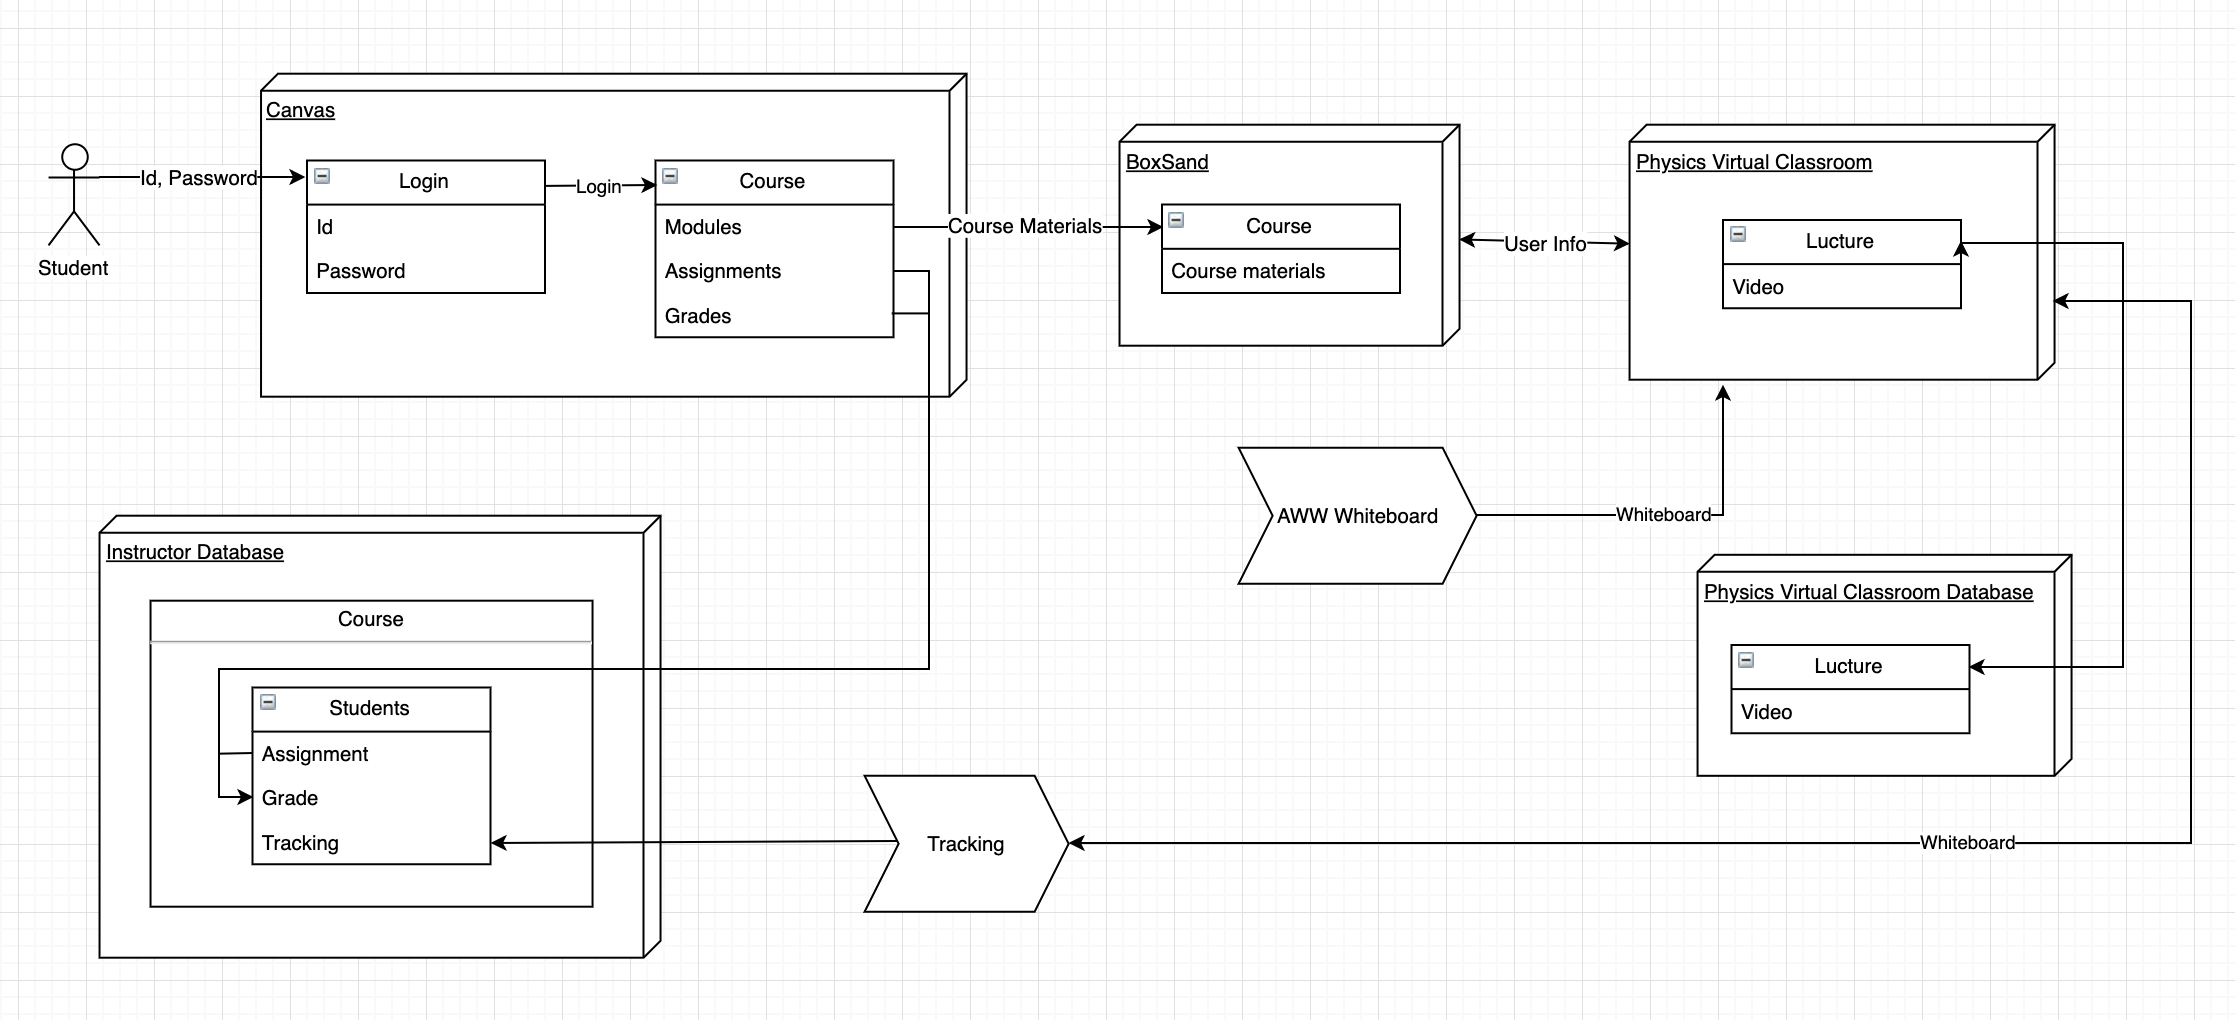
\includegraphics[width=0.9\textwidth]{{Design_Document/UML1}}
                \caption{Entire Project UML}
            \end{figure}

\newpage
        \subsubsection{Entire Project ERD}
            \begin{itemize}
                \item Student: A student has a unique user ID and password.
                \item Login Database: If a user ID and password match, a student can access to courses.
                \item Canvas: Canvas is the hub of the data exchange.
                \item BoxSand: BoxSand send and receive course materials and user information from Canvas
                \item Physics Virtual Classroom: This sends and receives lecture contents from Physic Virtual Classroom Database.
                \item Physics Virtual Classroom Database: This database includes lecture contents.
                \item AWW Whiteboard: It provides whiteboards to Physics Virtual Classroom.
                \item Instructor database: It contains Canvas data. Whiteboard tracking reports are also saved in here.
                \item Tracking: It receives whiteboard and then converts to tracking reports.
            \end{itemize}

            \begin{figure}[!ht]
                \centering
                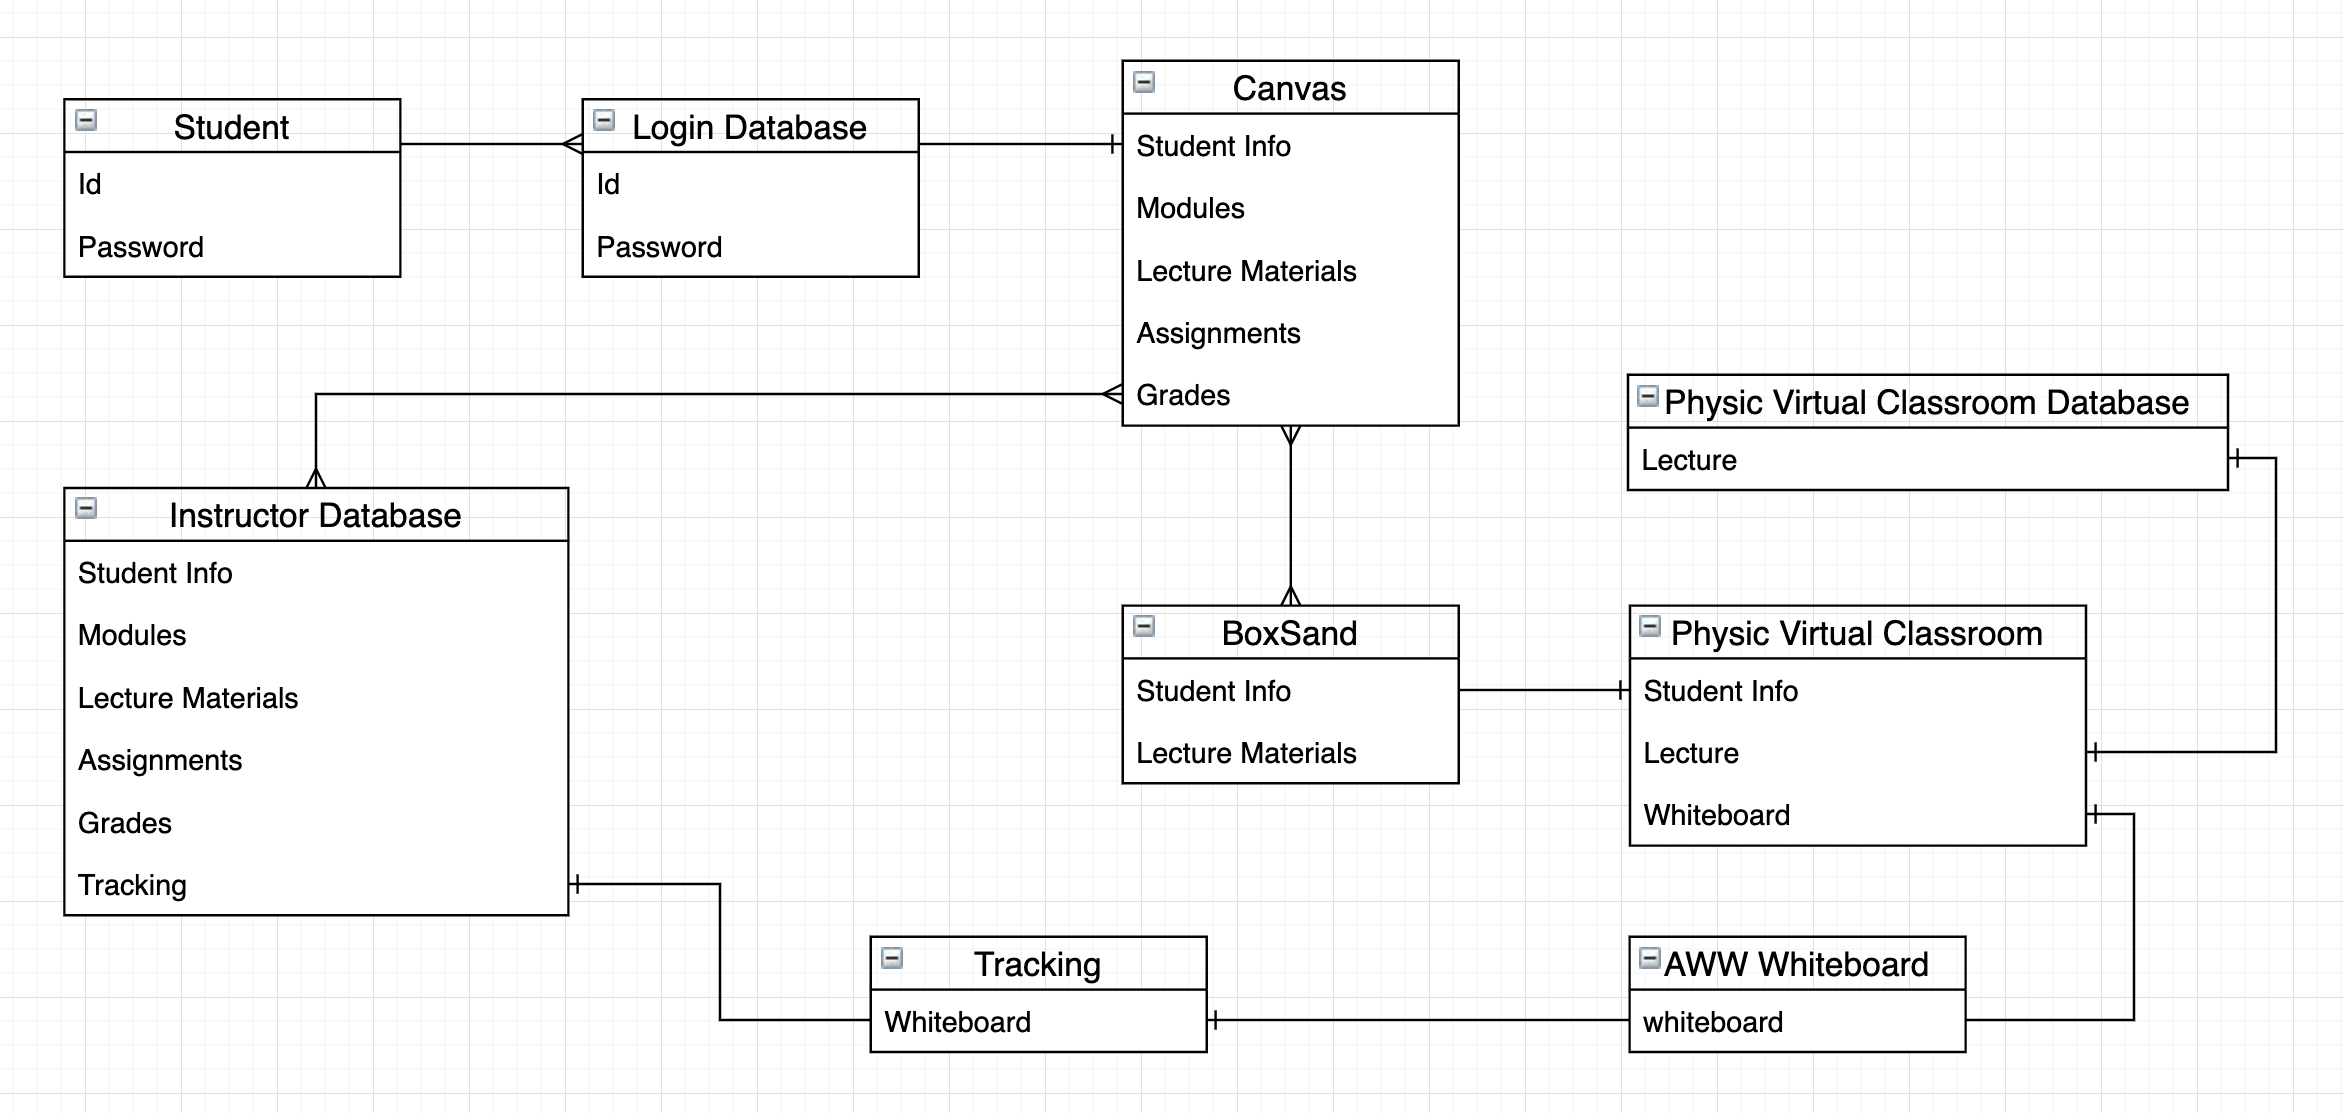
\includegraphics[width=0.9\textwidth]{Design_Document/ERD1}
                \caption{Entire Project ERD}
            \end{figure}

\newpage
        \subsubsection{Physics Virtual Classroom UML}
            \begin{itemize}
                \item Physics Virtual Classroom: This is the online live lecture page. Instructors upload YouTube Live lectures on this page. Students take lectures and work on questions together during lectures.
                \item Physics Virtual Classroom Database: Lecture contents are saved in this database. Physics Virtual Classroom page loads lectures from this database when students access to the web
                \item AWW Whiteboard: It provides a shared whiteboard to students during live lectures.
            \end{itemize}

            \begin{figure}[!ht]
                \centering
                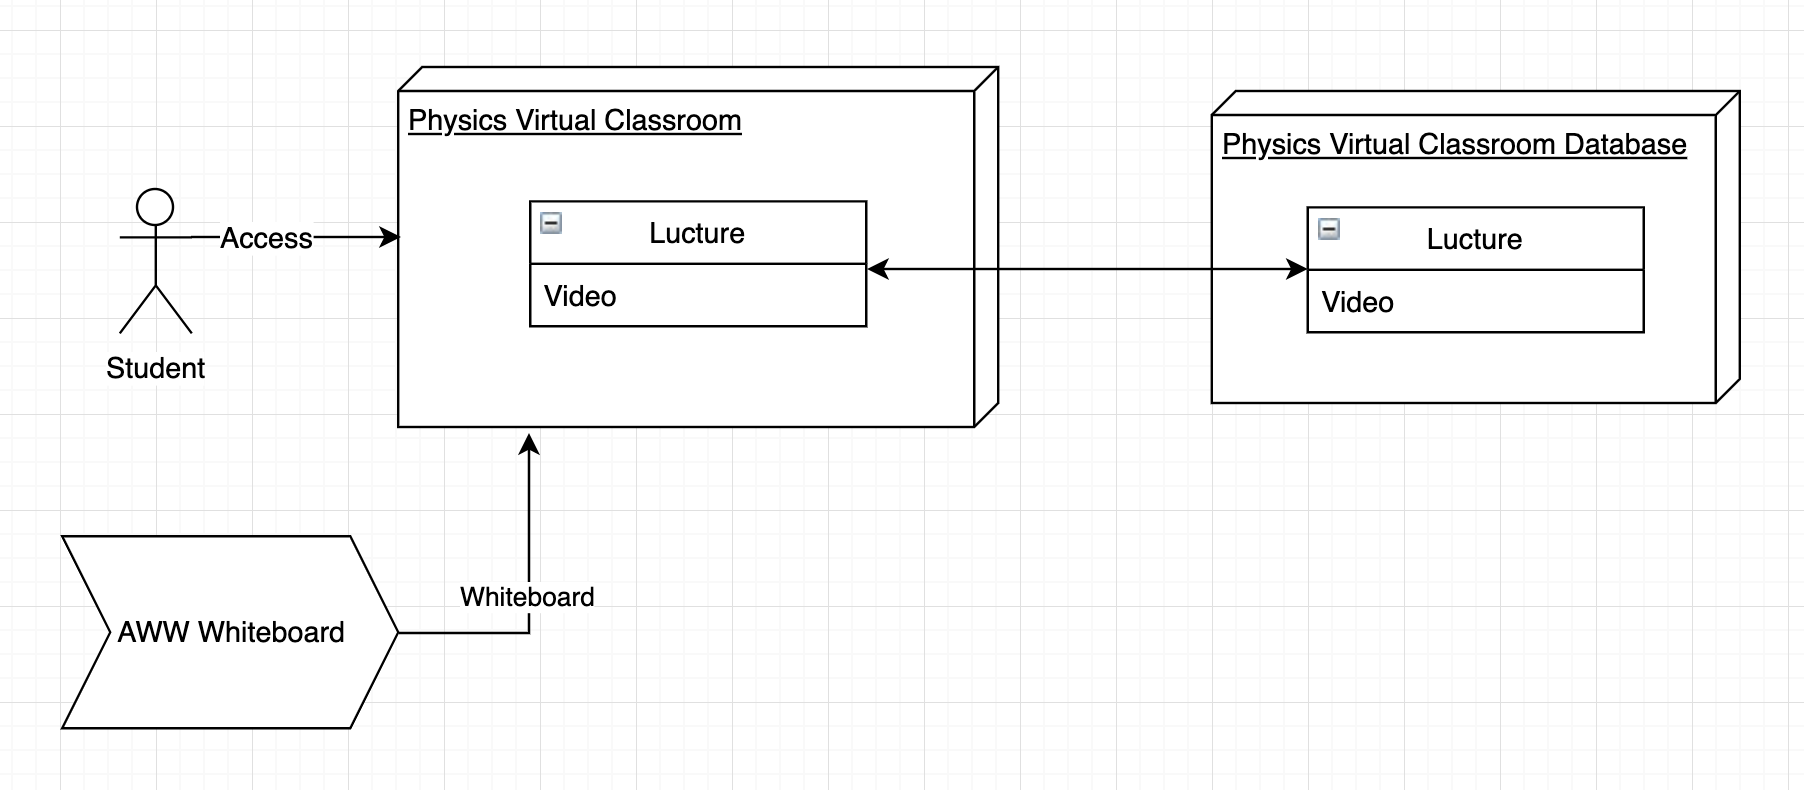
\includegraphics[width=0.8\textwidth]{Design_Document/UML2}
                \caption{Physics Virtual Classroom UML}
            \end{figure}

        \subsubsection{Physics Virtual Classroom ERD}
            \begin{itemize}
                \item Physics Virtual Classroom: This is a web page which students take live lectures.
                \item Physics Virtual Classroom Database: Database saves entries web page information. Not only lecture contents but also structure, theme, modules, and configuration are saved on it.
                \item AWW Whiteboard: AWW provides whiteboards to Physics Virtual Classroom. Students write and draw something during the lecture activity session.
            \end{itemize}

            \begin{figure}[!ht]
                \centering
                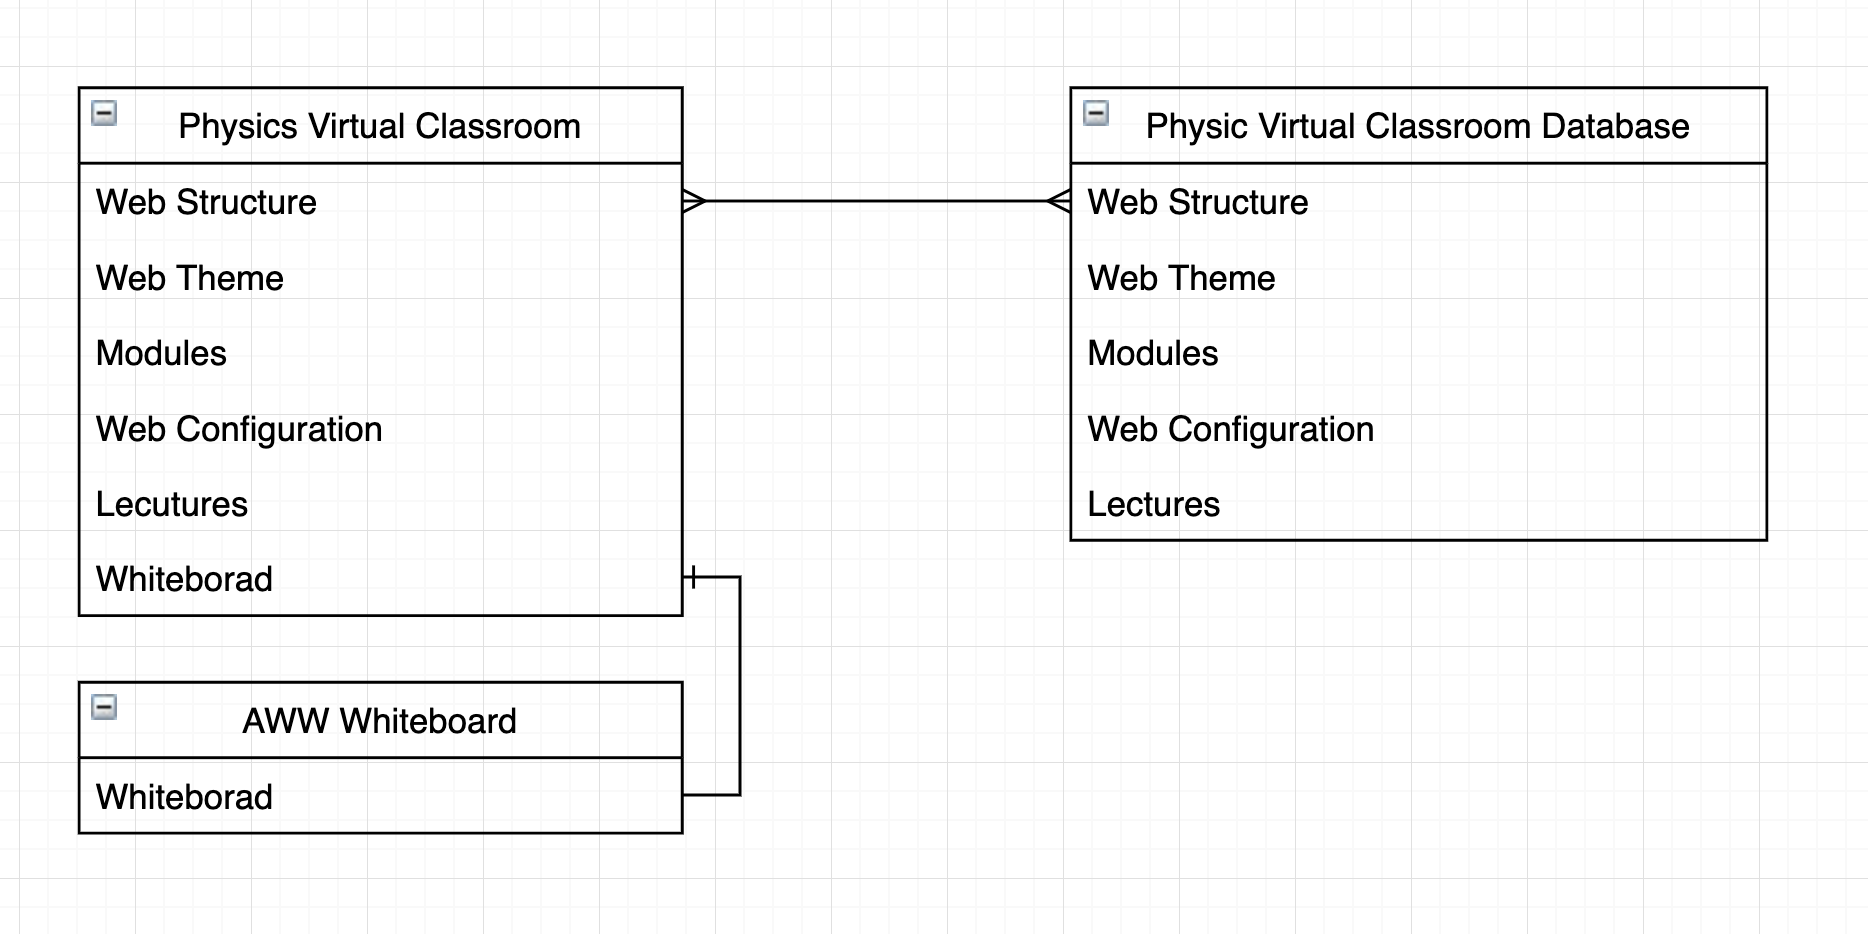
\includegraphics[width=0.7\textwidth]{Design_Document/ERD2}
                \caption{Physics Virtual Classroom ERD}
            \end{figure}

\newpage
    \subsection{Interface and Functionality}
        \subsubsection{Load the Physics Virtual Classroom Page}
            Students can access to Physics Virtual Classroom page by URL. Web recognizes access. Then query data from Physics Virtual Classroom database which is a MySQL database. Web Structure, appearance, and configuration are saved on a MySQL database. Web gets this information to build the Physic Virtual Classroom page. Then return this page to students.

            \begin{figure}[!ht]
                \centering
                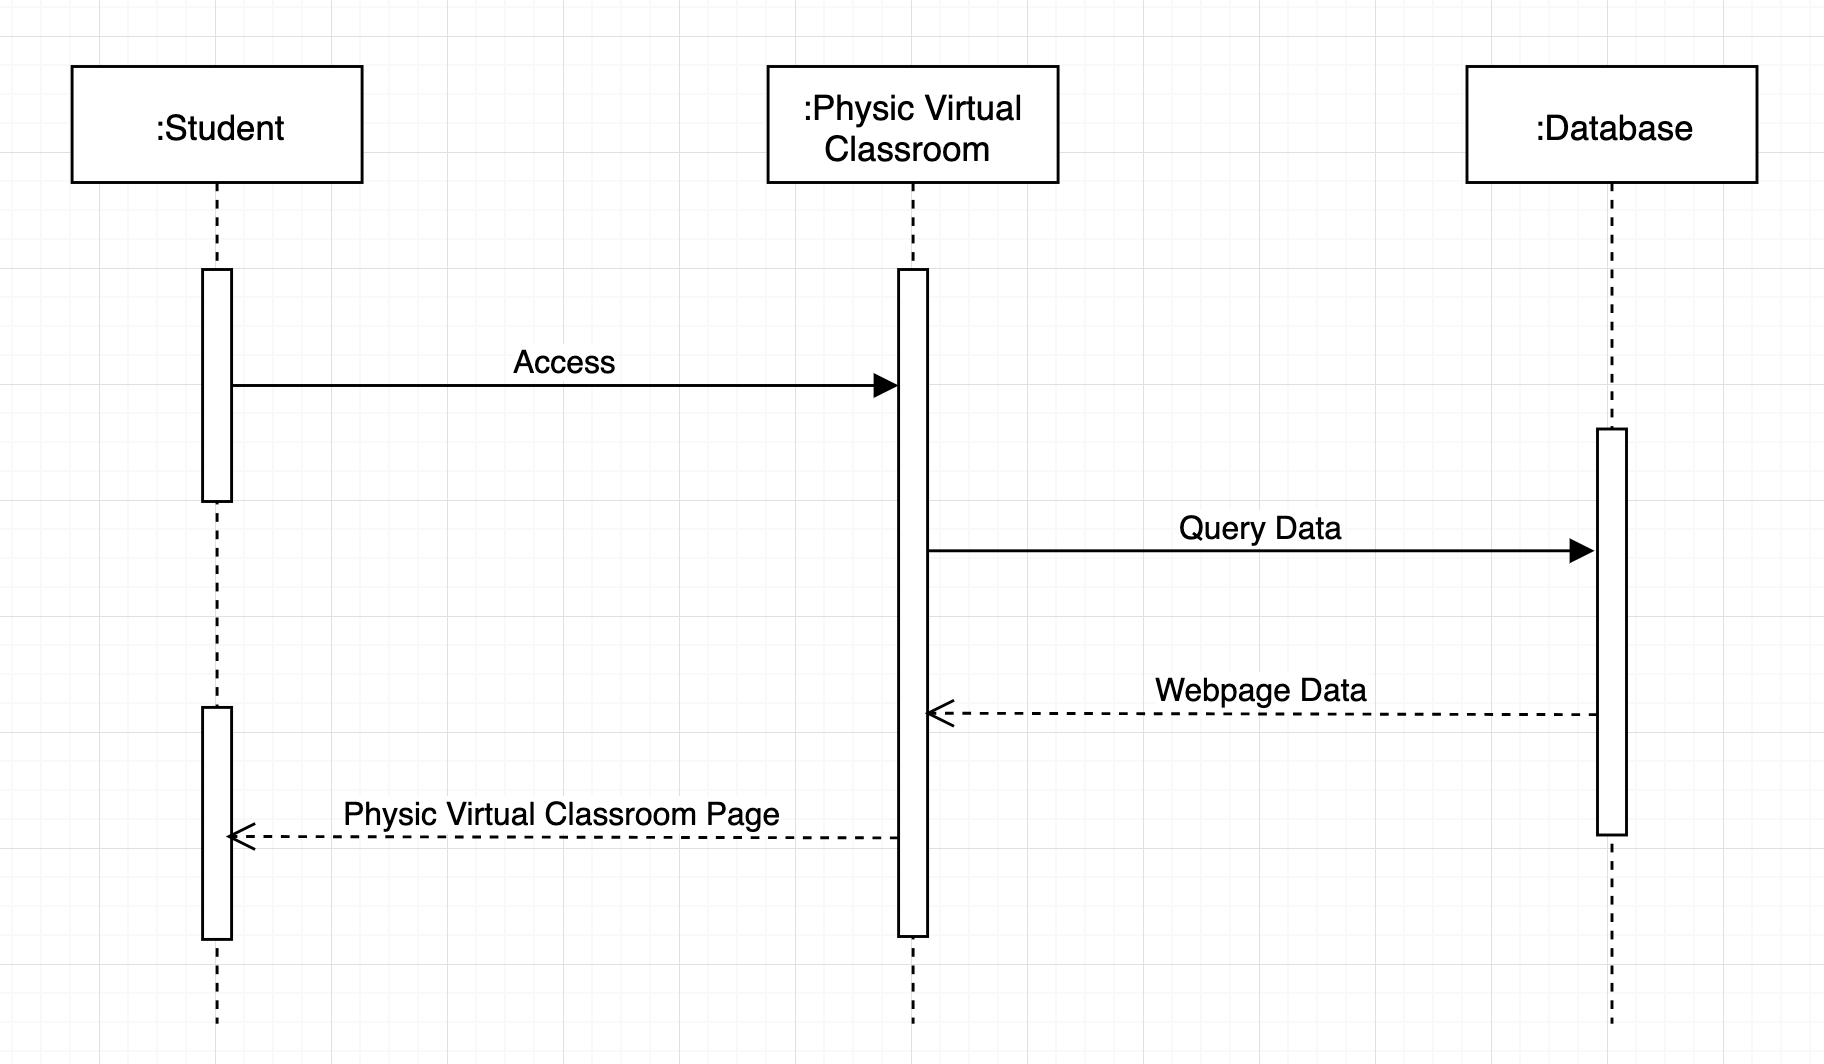
\includegraphics[width=0.7\textwidth]{{Design_Document/SD_Load}}
                \caption{Sequence Diagram: Load the Physics Virtual Classroom Page}
            \end{figure}

        \subsubsection{Add a live lecture}
            Instructor fills out the lecture content from. Then, he clicks the save button. Physics Virtual Classroom page sends this content to the database. This data is saved into a MySQL database. Database sends web page data to the Physics Virtual Classroom page. Then, the page is reloaded. Instructors and students can see added lecture.

            \begin{figure}[!ht]
                \centering
                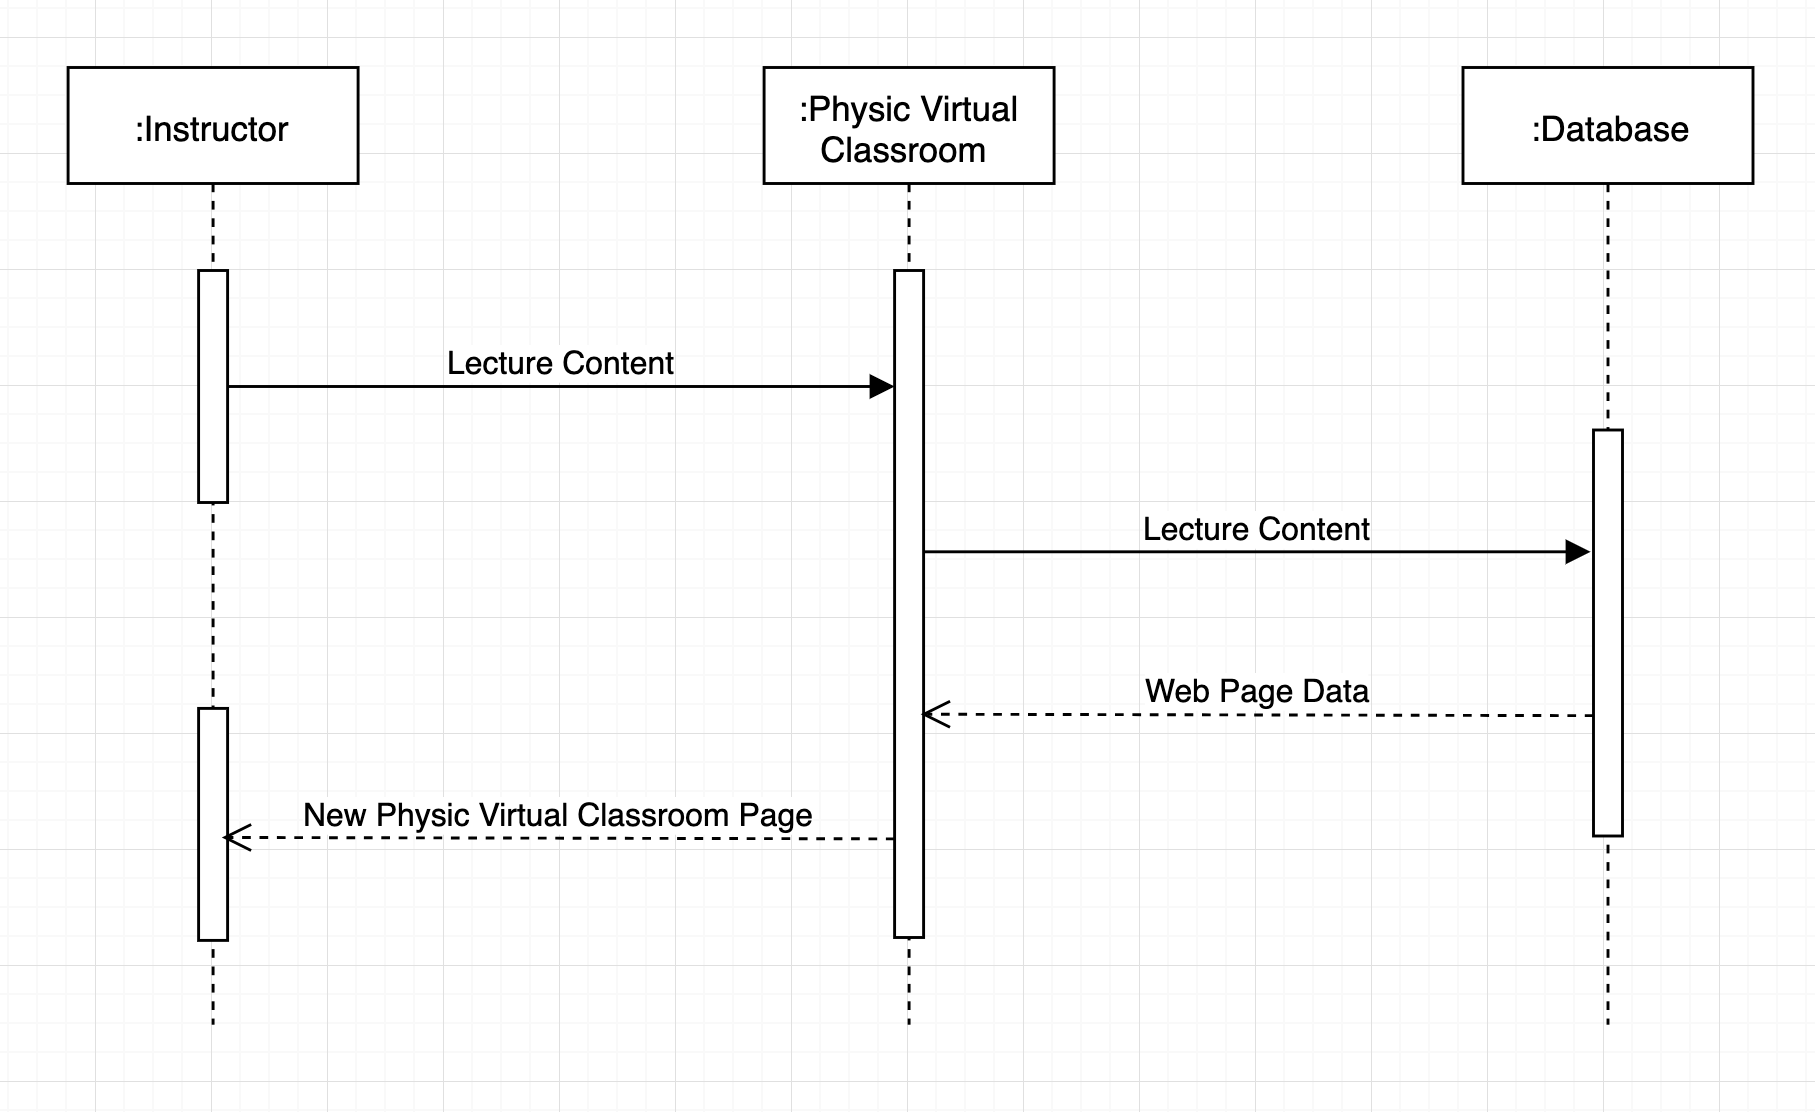
\includegraphics[width=0.7\textwidth]{Design_Document/SD_Add}
                \caption{Sequence Diagram: Add a live lecture}
            \end{figure}

        \subsubsection{Load a Whiteboard}
            Physics Virtual Classroom page query a whiteboard to AWW Whiteboard during live lectures. Then, AWW Whiteboard returns a whiteboard.

            \begin{figure}[!ht]
                \centering
                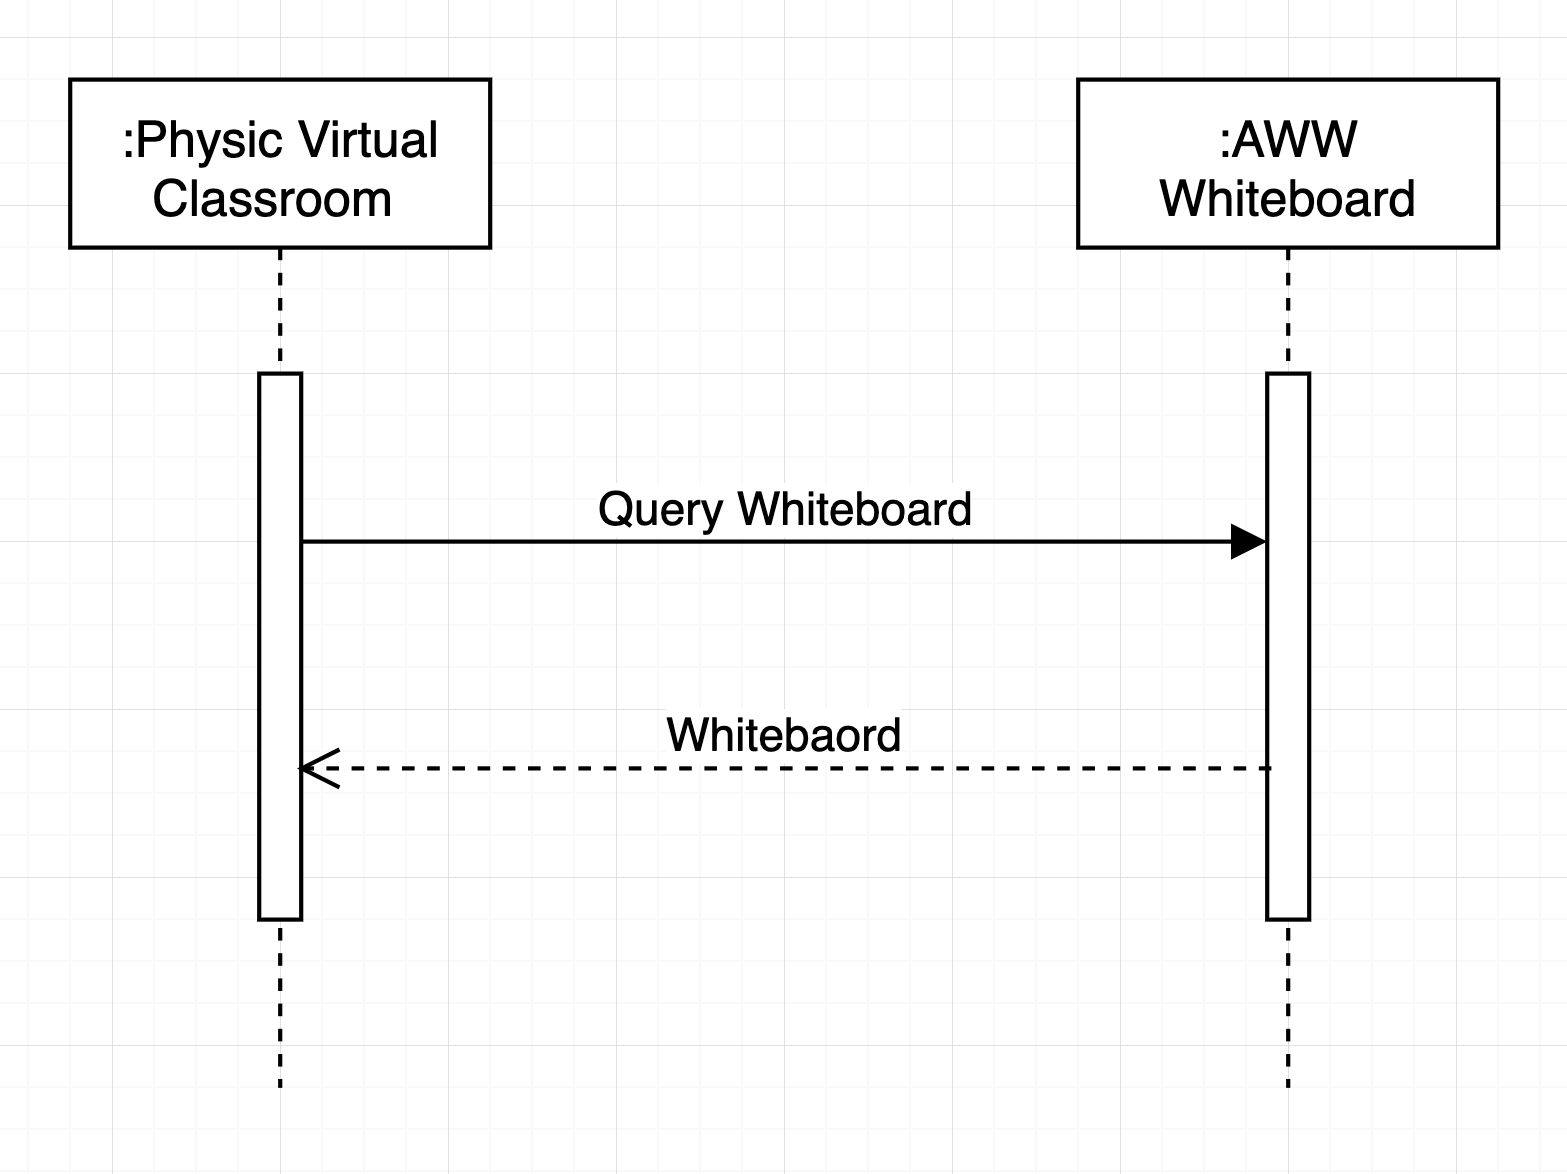
\includegraphics[width=0.4\textwidth]{{Design_Document/SD_WB}}
                \caption{Sequence Diagram: Load a Whiteboard}
            \end{figure}


    \subsection{Database}
        The database is going to be an integral part of the software because our main goal is to enable the instructors to schedule lectures on the Physics Virtual Classroom website and allow students to watch lectures. The information of the lectures that the instructors uploaded should be moved to the backend and stored in the database. This website will be created on the Drupal server. Drupal uses MySQL as the database, so the information of the lecture input must be stored in the MySQL database. The data will be stored in a related table so when students access the Physics Virtual Classroom website, the server will load the data.


    \subsection{Concerns and Constraints}
        \subsubsection{Using a new framework as our development environment.}
            We will use Drupal as our development environment. It was a suggestion of our head programmer. Due to the code, we had from another development team, had some issues, we were unable to continue working with the code. Therefore, our head programmer suggested Drupal. Drupal is an open-source CMS (Content Management System). There are several powerful advantages to using Drupal in our development environment. Mostly, other developers, who aren’t student developers, but full-time developers, in the Physics Virtual Classroom have been working with Drupal. So, they can maintain and work on this project once our part of the project is done. However, our team hasn’t used Drupal before, so we expect it will take time to learn. Moreover, in general, Drupal is unstable when is under development at times. This is due to the environment of Drupal. The developers can add modules to Drupal (which means you can add some functionalities to the website), but not all module guarantee compatibility with each other. Therefore, we need to work on adding modules locally first, and we can proceed if the job is safe to do. To sum it up, we expect there will be some learning curves to know how to develop the website by Drupal.

        \subsubsection{Some limitations on the whiteboard.}
            Students will have a couple of break-out sessions while they are taking lectures. They will go to the whiteboard and work with some of the other students. However, since the number of students, who will be taking the course, will be more than 100, the whiteboard will be needed many. We are thinking of each whiteboard has 4-5 students, and this will be the primary concerns of project teams, who will work on the project after our project is finished. Our system will have only one whiteboard even if 100 students are taking one lecture. To resolve this issue, we need to figure out how we can control users by their account. We will build to see the list of current users so that the next project team can work on this smoothly.

        \subsubsection{Server Management}
            Our server will be running on Ubuntu. We expect more than 200 students will use the website at the same time. Therefore, it is important to ensure that the server is running reliably.

        \subsubsection{Security \& other concerns}
            The goal of the whole project is to make a website that will help students to learn Physics a better and efficient way. Therefore, the website may be able to connect to Canvas, which is mostly used by students at Oregon State University. In that case, we should consider security as the primary concerns. More, we’ll use the student’s information in our database, so we need to take care of their sensitive data well.

     \subsection{Conclusion}
        In conclusion, the Physics Virtual Classroom project is a web software which allows students to collaborate in real-time. It lets students communicate online by offering a web-based chatting system. The whole website divides into three design parts which are the main page, the lecture page, and the whiteboard page. The main page will have a calendar that will show each lecture when is due. The lecture page will show the list of lectures and its descriptions. The whiteboard page will load the API from AWW. Students will go back and forth between a lecture session and a break-out session. Every lecture will be offered in live, and students may be able to re-take whenever they need to. Physics Virtual Classroom is the new style of the education program. It will replace the online physics assignment system. The virtual classroom project is expected to improve student learning efficiency.

     \subsection{Gantt Chart}
        \begin{figure}[!ht]
        \centering
            \includegraphics[width=0.8\textwidth]{{Design_Document/chart}}
            \caption{Gantt Chart (2018 Fall Term)}
        \end{figure}

        \begin{figure}[!ht]
        \centering
            \includegraphics[width=0.8\textwidth]{{Design_Document/chart2}}
            \caption{Gantt Chart (2018 Winter Term)}

        \end{figure}

        \begin{figure}[!ht]
        \centering
            \includegraphics[width=1.0\textwidth]{{Design_Document/chart3}}
            \caption{Gantt Chart (2019 Spring Term)}
        \end{figure}

\clearpage
\section{Tech Review}
    \subsection{Yeongae Lee}
        \subsubsection{Introduction}
            The purpose of the whiteboard program is to allow students to collaborate their work with other students. Collaboration with peers will allow students to learn about various ways to solve problems. AsyncSync’s client expects an executable whiteboard program in the real world, hence it should work well on the existing BoxSand webpage. Furthermore, we are also looking to implement it on the Canvas website. Our client expects this program to save students the cost of paying for private programs such as Mastering Physics, therefore we also considered cost while designing it. Before designing the program, coders have to search for most suitable and effective softwares that fits the purpose of our intended program. Hence, my role will be to search for the most fitting technologies and software in terms of purpose, quality and cost. Competitive softwares have both strong and weak points, so this paper will introduce the advantages and disadvantages of diverse whiteboard programs, front-end frameworks and chat clients.

        \subsubsection{Whiteboard}
            Implementing whiteboard on the BoxSand website is our main goal of the project. In order to do so, we must carefully identify the conditions of an effective whiteboard tool. First, our goal is to minimize cost so we have to consider the price to implement the whiteboard function on the BoxSand website. Secondly, functions of whiteboard should be taken into account. If the purpose of a whiteboard is to just share solutions, it does not need to provide complicated drawing tools. Too many unnecessary functions might give a bad impression on users, deeming it not user-friendly. Finally, the qualities of whiteboards should be taken into consideration. Whether the functions perform effectively is the most important factor. We have to test the program functionality on various platforms such as laptops, tablets, Windows, and Mac. \cite{Online Whiteboards}

            \paragraph{AWW App}
                In my research on whiteboard programs out there, I found that AWW App is faithful to the basic functions. It allows more than one user to work on a board and contains the AWW board with a dot grid, which helps to align pictures and text. AWW has similar functions in comparison to Whiteboard Fox, which will be introduced next but it is visually more appealing than that of Whiteboard Fox. The AWW App provides basic drawing tools such as drawing, eraser and copy and paste functions. One disadvantage of AWW is that it lacks sophisticated tools. If a client wants more advanced collaboration, it might be not sufficient. According to the official AWW website, it has a free version. However, it is only for the individual users without the collaborative function. Aside from the free version, AWW App also provides an organization and a custom version, which will be our focus as they contain the collaborative functions. These are priced at \$ 3.24 per year which is used for educational purposes which aligns with our goal. However, as we have to implement it on the BoxSand website, a custom or organization version would be more appropriate. To be sure, it would be best to contact them and ask for their opinion on which is a better option for our project. \cite{AWW APP Price}

            \paragraph{Whiteboard Fox}
                Looking at the second whiteboard program, Whiteboard Fox is a simple and fast virtual whiteboard as it does not require setup or installation to run the program. It is similar to the AWW App in terms of the simplicity of the drawing tools. The only difference is that Whiteboard Fox has a copy all feature that allows users to copy all drawings to the clipboard at once. In terms of features, there are not plenty but it is still a popular online whiteboard because of its fast Syncing and simple usage. The biggest strength of Whiteboard Fox is that it instantly shows all the changes on the right side of the screen in real-time. To add on to that, it is also a tablet-friendly software. The price description is not found on the webpage, so it is questionable whether they will allow us to use the software for our BoxSand project. Hence, we would have to contact them for more assistance.

            \paragraph{RealTime Board}
                In contrast with the previous two whiteboard programs, RealTime Board is a much higher-level whiteboard. It supports various collaboration works, provides basic drawing tools and enables cloud network collaboration. Furthermore, it provides diverse templates; users can create charts, tables, and various note cards. In terms of advantage, the advanced functions are the greatest strength of RealTime Board. For instance, whiteboards can be saved as image, pdf and allows users to save their work on Google drive. Best of all, It has a free version that supports up to a maximum of three members in a board. The price increases if more members would like to be added into the board. We will contact them to inquire more details. \cite{RealTime Board Price}

            \begin{tabular}{ | p{0.2\linewidth} | p{0.2\linewidth} | p{0.2\linewidth} | p{0.2\linewidth} | } \hline
                 & AWW & Whiteboard Fox & RealTime Board \\ \hline
                Cost & Educational version & No information & Average \\ \hline
                Functions & Basic drawing tools & Basic drawing tools & Basic drawing tools Template \\ \hline
                Platform & Windows, Mac & Windows, Mac & Windows, Mac \\ \hline
            \end{tabular}

        \subsubsection{Front-end Framework}
            There are a few aspects to consider in choosing a front-end framework. First, coders’ ability is important. Novice coders are better at deciding frameworks which provide many useful widgets and templates as they only require minimum coding skills. Secondly, users have to take into account the expected outcome appearance in different platforms. Frameworks are different depending on platform. If coders want to develop a unique website outside of normal standards, it would be helpful for them to choose a front-end framework which supports high level customizing. Finally, coders have to consider provided CSS preprocessors. Different front-end frameworks provide different CSS frameworks. It is better to decide a front-end framework which provides CSS preprocessors which we are comfortable with. \cite{Front-end Frameworks}


            \paragraph{Bootstrap}
                Bootstrap is the most widely used open source front-end framework. Bootstrap includes HTML, CSS, JavaScript and JS. It supports both LESS and Sass CSS framework. It is a framework that complies with responsive web design standards, so this is suitable with all different sizes and complexities of web development. Bootstrap provides consistent results between browsers, allowing end results to look the same on provided platforms and browsers. Bootstrap is one the most popular framework, so it is frequently updated and new features are frequently added to it. Moreover, Bootstrap supports the latest versions of Chrome, Firefox, Internet Explorer, Opera, and Safari. Despite the many advantages, it is not compatible with all coders. For example, Bootstrap contains a customary framework, so coders who wishes to deviate from standards have to spend much time on coding. Bootstrap websites also follow standard templates. Therefore, most websites which are built with Bootstrap might look similar to each other. Lastly, Bootstrap includes a lot of excessive tools which are not frequently used, slowing down the loading speed.

            \paragraph{Foundation}
                Foundation is a high-level open source framework. It provides Sass CSS preprocessor. It is an ideal front-end framework for responsive website development. It is a framework which requires high customization ability, so this framework is often used to build unique websites that do not get stuck in a rut. Foundation also has a strong flexible grid system like Bootstrap. What stands out when comparing it to other frameworks is that style classes are already included, so it does not need to include classes on the code, preventing the size of the CSS file from being lengthened. However, foundation’s advantage can be its disadvantage as customization could be a complex process for beginners, it could take extra effort and time for them to lean it.

            \paragraph{Semantic-UI}
                Semantic-UI is also one of the often-used open source front-end framework which supports LESS preprocessor. Similar to Foundation, customization ability is also required. The strongest point of Sematic-UI is that it is well arranged with Each component configured with its own file, thus allowing users to easily load components and reduces file size and loading time. Semantic-UI is appropriate for modern elegant design websites. Disadvantages of Semantic-UI is that it utilizes JavaScript customization solution, so Semantic-UI users have to familiarize with JavaScript beforehand. Aside from that, it provides fewer classes than Bootstrap and Foundation.

        \subsubsection{Chat Client}
            Communication in a group is important for collaborative assignments and Chat Client is a method to allow that. Our primary purpose is to implement a whiteboard function on the BoxSand website. For that, we have to consider features of chat software. A client’s opinion is important to decide on a chat software. It depends on the preference of a client to decide on a chat software that supports either basic chat functions or one that provides more ancillary features. Programs that provide additional functions are normally more expensive than the ones with basic functions. So, cost should be allocated depending on the need of additional functions or not.

            \paragraph{Slack}
                Slack is a chat program that already forms a lot of users. 77\% of the Fortune 100 uses Slack. Slack has aribnb, Target, trivago, CapitalOne as clients. Among the programs which will be introduced from now on, only Slack has a free version. Slack provides Cloud, Windows, and Mac OS platform. Slack does not include advanced features such as Geo-targeting, offline form, screen sharing but it is fast. Even if it accommodates multiple users on one channel, it does not have running slow problem. Simple and fast is the greatest strength of Slack.

            \paragraph{Chatwing}
                Chatwing is a Live chat platform widely used on websites and mobile devices, providing to more than 3 million websites worldwide. In terms of functionality, users can add chat boxes and widgets on their websites and allows users to easily customize the chat box design, allowing a smooth integration with user websites. Lastly, it also supports Windows, Mac OS, iOS, and Android operating systems. According to the official website, the price is \$250 per month for enterprise use. \cite{Chatwing Price}

             \paragraph{LiveAgent}
                LiveAgent is a popular live chat software popular amongst big companies such as BMW, Yamaha, Huawei, and Orange. LiveAgent provides more diverse features than Slack, having more than 170 features. Besides that, it is easy to use and has a user-friendly interface. In terms of disadvantage, it only works on the cloud platform and lack customization settings, so It can be difficult to set up CSS that works well with a website. In terms of price, it is \$39 a month based on the official site but the detailed price can be known by contacting them. \cite{LiveAgent Price}

            \begin{tabular}{ | p{0.2\linewidth} | p{0.2\linewidth} | p{0.2\linewidth} | p{0.2\linewidth} | } \hline
                 & Slack & Chatwing & LiveAgent \\ \hline
                Cost & Average low & Average & Average high \\ \hline
                Free Version & Yes & No & No \\ \hline
                Platform & Windows, Mac, Cloud & Windows, Mac & Windows, Mac, Cloud \\ \hline
                Customization & Average & Average & Average low \\ \hline
            \end{tabular}

        \subsubsection{Conclusion}
            To conclude, our BoxSand project aims to implement a real-time collaboration software. Students will be able to learn various ways to solve problems by collaborating with peers. Our team considers various technical components such as whiteboard programs, front-end frameworks and chat clients. We will also compare the features of the programs such as quality and price and select the one that work best for us. BoxSand is a new style of the education program which will replace the online physics assignment system. Our project goal is to improve student learning efficiency while conserving their budget.

    \subsection{Jaehyung You}
        \subsubsection{Whiteboard}
            The whiteboard is going to be a main part of the project. The problem of many whiteboard, which are currently in use, is the general-purpose use rather than the educational purpose. Our goal is to enable all students to use the many online shared whiteboard features that are currently available only by paid. Our team will try to implement all the necessary features of the shared whiteboard for educational purposes, but we will keep everything simple and intuitive for every student, who is going to use. In this review, I’ll focus on reviewing the overall functionality, because the details of our project may change as the project progresses.

            \paragraph{AWW Whiteboard}
                AWW, which stands for A Web Whiteboard, this whiteboard system shows many of the features of the online shared whiteboard, that is going be developed by our team. It also has the feature that anyone can invite other people to edit or view the whiteboard, so they can increase their productivity. However, the biggest problem of this application is many essential features are not free, which could be useful for students for collaborating their work. This means the user could see some commercial advertisements on the board, which is not good for educational purposes. Nevertheless, the application provides an intuitive and easy-to-use API, which would be very helpful for future progress. More interesting feature of the application is that the user can have the unlimited online white-board. It means the whiteboard can’t run out of space. This feature will give a high productivity for several people working on a small screen. \cite{AWW}

            \paragraph{Tutorialspoint Online Whiteboard}
                 This system shows almost final appearance of the project we are aiming for. The application gives users many features without showing advertisements and requiring any kinds of payments. The best feature when compared to other applications, it has more educational features. First, the process or method of inviting other users to your workspace is very simple and convenient. Even it has a voice chatting and a regular chatting system, so it helps to keep everything going smoothly in the way they want. It also has a tutoring system, which is one of the features we want to make it eventually, so any users can get help from the other users or tutors. However, this application only allows few colors to draw, which isn’t ideal while several different students are working in the same workspace. It may bring confusion to other students unless the program indicates who draws what. Still, this program will be able to give us a good direction in making our project. \cite{TW}

            \paragraph{Ziteboard}
                This system has most main features for the online shared whiteboard, like the above. However, this system has a more diversity and productivity feature that is a sticky note. From time to time, many users want to leave a mark that indicates what the user really means. So, this feature could be very helpful while students are working with a difficult equation or something is not clear. Compared to the other two application, this one has more faster switching jobs. For example, if the user wants to move the board while he/she is drawing, the user simply use a scroll and move the board. Afterwards, the user can draw simply by double-clicking the board. This kind of feature will increase student’s work efficiency. \cite{Zite}

            \paragraph{Summary}
                Those whiteboards, which are already developed online, are great example that we are aiming for our project. In the meanwhile, they still have some unnecessary features that isn’t good for educational purposes. So, our team should only take good advantage from those, and we have to make sure that there is any inconveniences for students to work.

                \begin{center}
                \begin{tabular}{ |c|c|c|c| } \hline
                     Options & Advantage & Disadvantage & Note \\
                     AWW & Simple API for using, Core features for sharing & Pay for using all features & \$7.5/mo per 10users  \\
                     Tutorialspoint & Free, Simple Appearance & Lack of tools for drawing & API not provided\\
                     Ziteboard & Productivity features & Pay for using all features & -\\
                     \hline
                \end{tabular}
                \end{center}

        \subsubsection{Database/Cloud-based System}
            Database is good way to store data, which is a tracking information of students’ work. As one of our requirements of this project is having a tracking system of students’ work so that they can have a reasonable grade, or the professor can give them a feedback. Since the method of storing students’ work isn’t defined yet, the type of databases (or DBMS) will be differed as the project progresses. It would be better to use cloud-based database, since we will store pictures or videos of students’ work.

            \paragraph{MongoDB}
                First, MongoDB is an open-source database, and it is developed in C++. It shows a great scalability and performance, it is a Document-Oriented database system. It supports fully indexing, so it could be a good choice if we are going to store tracked students’ work as an image. This is because it has a great performance on reading and writing data, so it can handle a big caching or huge traffic of data. Why the reason for MongoDB isn’t good for storing a video is that it only allows only small amount of size of the data. So, if we are going to store a lot of images or a video, MongoDB wouldn’t be ideal. Moreover, it is also a memory mapped file, which is a database using a file engine, so every memory managing is by the operating system we use. Therefore, the performance, that we expect, can’t meet our expectation if our system isn’t good enough. However, depending on how we store the data, MongoDB can be a good choice. \cite{mongo}

            \paragraph{Microsoft Azure}
                It is more like cloud-based system rather than the traditional database. However, it could be a great choice if the tracking file is going to be an image or a video. Since the size of those data will be tremendous, Azure can handle the process faster than any other database managing system (DBMS). Especially, for data storage, there is a service which is called “Blob Storage”. It is a REST-based object storage for unstructured data. Moreover, it could easily connect to the other database system, so managing the data is more efficient and convenient. However, if the data gets larger, the pricing point would be going higher, which isn’t good for the client and us. For this reason, it will be necessary to manage and erase the data at regular intervals of time. \cite{azure}

            \paragraph{MySQL}
                This is the most common-use database in the world. It is a relational database system, and it also allows multi-users and multi-threads. Most importantly, it gives the user various API for C, C++, Java, PHP, and etc. It is also free to use, because it is from an open-source library. Moreover, it uses the standard SQL form, so every team member can use MySQL without any prior knowledge of it. So, if we are going to store the data by a different format than images or videos, MySQL is good choice to go. This is because it is simple and fast enough to handle a huge data. However, it isn’t easy to change particular data model because the data table is less flexible than other data base system, like MongoDB. However, it still has a great performance and secure features, so it can be a good choice depending how the data will be stored. \cite{mysql}

            \paragraph{Summary}
                There are tons of database/cloud-based on the market, but finding a right database isn’t easy step for every project. Since we haven’t figured out how the tracking data would look like, the choice of database would be differed at any point. However, we should be aware of the advantages or disadvantages of these database system or cloud-based system, so we can progress our project more smoothly and flexibly.

                \begin{center}
                \begin{tabular}{ |c|c|c|c| } \hline
                     Options & Advantage & Disadvantage & Note \\
                     MongoDB & Great performance for reading and writing & Not good for handling many images and videos & - \\
                     Microsoft Azure & Good for handling many images and videos & Pricing point would be high & -\\
                     MySQL & Easy to use and handle the data & Not good for handling many images and video & -\\
                     \hline
                \end{tabular}
                \end{center}

        \subsubsection{WebSocket}
            WebSocket is a communication protocol by using one of the TCP connection. In other words, there will be a continuous connection between the web browser and the server by WebSocket. It means that a persistent connection is established between the client and the server, so both can send data at any time. This feature will be required our project, since we are going to use a chatting system or a voice chatting system on the whiteboard. Those chatting systems requires an immediate connection and response. Therefore, WebSocket is a great choice for those system. Since the specifications of this WebSocket are internationally uniform, we will look at how we will implement this feature by languages.

            \paragraph{Socket.io}
                Socket.io is developed by NodeJS. It is the most basic way to implement WebSocket. It requires npm (Node Package Manager). More precisely, Socket.io aims for developing a real-time chatting system by using WebSocket. This is one of great tools that has been optimized to develop the real-time chatting system. Most importantly, this will enable all the browser, which doesn’t support WebSocket, to be able to use WebSocket feature. For example, most browsers, nowadays, support WebSocket, but IE only supports it after its version 10. \cite{si}

            \paragraph{Flask-SocketIO }
                Flask-SocketIO is a flask application that access to low latency communications between the clients-side and the server-side. The flask is a micro web framework in Python. This micro web framework includes many advantages, because it doesn’t require specific tools or libraries. Which means, it could be implemented any kind of developing environment. Since Flask-SocketIO can allow that the client-side application can use any of the original Socket.io libraries in many languages, it may able to give us a bit more diversity for developing options to our project. This scalability of Flask-SocketIO will help us as the project progresses \cite{fs}

            \paragraph{ws}
                It is another a popular WebSocket library for JavaScript, especially Node.js. It also helps to manage connections under the WebSocket Protocol. Since Socket.io is much easier to use for developing a real-time chatting system, this one doesn’t seem to have any advantage to use. However, Socket.io is more focused on the real-time chatting system, while this one has more focused to the basic role of connecting client side and server side. It is also very simple to use and fast enough to implement the real-time chatting system. Socket.io is enough to develop the chatting system, however we could need to know this library in case we need to add more feature, which needs the connection between the client-side and the server-side, rather than just having a real-time chatting system. \cite{ws}

            \paragraph{Summary}
                WebSocket is a great tool for implementing the real-time chatting system. Like Socket.io, there is an already great library to use.  These WebSocket technologies play a crucial role in the workspace of students, because they need to go in the right direction of the right answer with immediate feedback from other students. Since what chatting system will be implemented on the whiteboard hasn’t decided yet, those options will be important choices in the future.

                \begin{center}
                \begin{tabular}{ |c|c|c|c| } \hline
                     Options & Advantage & Disadvantage & Note \\
                     Socket.io & Easy to use, great for the real-time chat system & - & Implementing voice \\
                     & & & chatting is tricky\\
                     Flask-Socket.io & Flexible on any developing environments & Except that, Socket.io is& -\\
                     &&better and easy to implement&\\
                     ws & Better library for connection between & Not easy as Socket.io  & It is running under\\
                     &Client and Server& & WebSocket protocol\\
                     \hline
                \end{tabular}
                \end{center}
\newpage
\section{Weekly Blog Posts}
    \subsection{Yeongae Lee}
        \subsubsection{2018 Fall Term}
            \begin{center}
            \begin{tabular}{ | p{0.1\linewidth} | p{0.8\linewidth} | } \hline
                Week & Contents  \\ \hline
                Week 2 & Week 2 is for deciding the project to work for the next 3 terms. I read all the project descriptions in detail. Then noted projects numbers which I am interested in. After, I listed projects which I am interested in. I checked the requirements for projects. Some projects required specific languages. Therefore, my ability is not fit with most of the requirements, I unlisted that projects. Through this process, I got my favorite 10 projects. Then I wrote reason to choose projects. I gave higher priority to projects which are easy to explain why I am interested. I completed a list of favorite projects. However, 10 projects are too much, so I randomly picked the last 2 projects. The future plan is after I am assigned the project, I will context group members and customer to build a detailed project.  \\ \hline
                Week 3 & In week3, we got a team, so I know what will I work on during the next three terms. I will create the BoxSand program. This week assignment is to write a problem statement document. I have to write about an outline of the project. Fortunately, the description for box sand program details enough. I added a few detail points which I think that it will be useful. The document is about my idea for this project, so it is too wide to start but there were not many difficulties. I met team members to take about the project. Our team just have a simple understanding of the BoxSand program. We will meet customer next week and built detail Plan for next week is meeting a client to get more information about the program.  \\ \hline
                Week 4 & We met the client this week Thursday. This is the first time to meet a client. The project was a little bit different from my thought. Therefore, it was a good time to figure out the project. A client has a great passion for the project. He also has a clear idea about it. We got detail information about the project during the meeting. The purpose of this project is super attractive. It will be a great tool for OSU students. We shared individual problem statements. We have writing due this week, so we shared the idea and came up with a group document. I got the metrics section to fill out. Writing it already submitted, so everything is going good so far. We have a group paper due next week, so we will meet a person who helps us to create the project. We will get server and coding informational about the project. Our customer is not in the Computer Science major or department, so he will help us to start actual coding.  \\ \hline
                Week 5 & This week had to write requirements document draft 1. However, the due date was changed so we got more time to work for this assignment. To write better requirements document, we had to get technical information about the project. We met Max who is a BoxSand program director. He is a coder who works with our client. He explained the technical side of the program. The online class is working on one of the boxes and function. That function should cooperate with our whiteboard function. Therefore, we have to clarify which prat for a function should we do and they do. Also, how can we make two functions work together without any problems? We got the foundation to write a paper during a meeting with Max.  \\ \hline
                Week 6 & We did not have a client meeting this week. It had but it was canceled. I will have a meeting with a client and online group who are already working on other function of BoxSand. I am confusing which parts online class will cover and which parts we will cover. It will be a great opportunity to check this part. Our team will prepare a question to ask them for a meeting. This week assignment is Tech Review writing. It spent more time than my expectation. It needs a lot of resource about software and platforms.  \\ \hline
                Week 7 & This week we had a meeting with a client. We could not meet other BoxSand team but it was a great opportunity to get information. It was 2hours meeting. They told us some software which we have to search before the next meeting. That software is used to create BoxSand web page. Therefore, we also have to search for it and learn it for projects. This week we have Tech Review Final paper due. I searched for software again. Then, I fixed Tech Review first draft to write a final paper.  \\ \hline
            \end{tabular}

            \begin{tabular}{ | p{0.1\linewidth} | p{0.8\linewidth} | } \hline
                Week & Contents  \\ \hline
                Week 8 & This week we do not have assignments and meeting. We did not quite do anything. We will have a meeting after Thanksgiving. I have to research the required program during the next two weeks.  \\ \hline
                Week 9 & Thanksgiving is on this week, so we had a long holiday. Therefore, we got a meeting before we had a long holiday. We will write the design document based on meeting information. Next week is week 10, so there have many assignments due, we will spend most of the time for those.  \\ \hline
            \end{tabular}
            \end{center}

        \subsubsection{2018 Winter Term}
            \begin{center}
            \begin{tabular}{ | p{0.1\linewidth} | p{0.8\linewidth} | } \hline
                Week & Contents  \\ \hline
                Week 1 & We missed one team member. We had four members but now we have to finish this project with three members. We met with Max who manages the technical part of the project. He asked us to implement the Whiteboard to  Canvas until next week. We will work that part until next week. Then, we will meet him again next week and report the current process.   \\ \hline
                Week 2 &  We got code last week but, we do not have authority to access code. This week we met the head programmer. He fixed code to allow us to run the code. We can run the program, so group members will meet this week Sunday and work on implementing whiteboard to BoxSand website. We will also take about the pre-draft poster. We have the first client meeting next week. Also, we will start to implement chat to BoxSand website. \\ \hline
                Week 3 & This week had an assignment which is a poster. We met on weekends are finished assignment. We will have a big client meeting. We will meet Online students who are working on this project and the client. That will be a great time to be clear what we have to do. Our project is kind of overlapped with  Online students work. Therefore, it is so difficult to figure out their part and our part. We have to have a client meeting to figure out it. We did not have the opportunity to meet them before, so we always got their idea form client.   \\ \hline
                Week 4 & This week we missed one member, so we have to finish the project with two people. I am a little bit worry about it but we have to finish the project. Since we have fewer members than other groups we will try to do most of part in this term. If we push it to the end, we might not finish the project. We have a  group meeting next week on Monday. I will start to do coding on that day. Also, we found a group to work poster critique together. This assignment is submitted. Rather than team member problem, we are ok. Everything is on the way.    \\ \hline
                Week 5 &  We have poster critique class this week, so we met with a different group and got advice, so we will progress the poster. We have to figure out how we can put 5 members in one whiteboard. We came up with the idea but before we actually implement it, we have to tell our head programmer. If he said it fine, we can start coding. Next week meeting is Wednesday. If there is a better way to put students on a board, we will get advice and change it. We also talked about the next writing assignment and we will work on this and next weeks.   \\ \hline
                Week 6 & Our group started to write winter term report. The due date was extended, so we have more time to think about it. We had a meeting this week with the head programmer. Our group will meet and do coding on this Saturday. We aim to write the code which allows the server to get user information who access to BoxSand from Canvas. This is the first step for grouping. We will figure out that part. Then we will work on break out users into a group during next week. We will have three different breaks out session, so we will also take about how to make different groups for each break out session in this week.   \\ \hline
                Week 7 & What we expected to do this week is be friendly with Drupal. We spend most of the time figuring out Drupal this week. This is a new tool for us. Also, it does not have any instructions online. Therefore, we got difficulties to use it. We depending on Drupal Document to developing our project. If it is not enough to solve the problem, we will get help from the head programmer. We had two meetings with him this week. Next week also will probably have one or two meetings to develop the project. Next week plan is doing an assignment and working on chat implementing.   \\ \hline
            \end{tabular}

            \begin{tabular}{ | p{0.1\linewidth} | p{0.8\linewidth} | } \hline
                Week & Contents  \\ \hline
                Week 8 & This week, we are working on bringing virtual class to Drupal server. I found out there is a module to implement it.  However, it does not quite work, so we are struggling with it. Maybe we will keep working on this next week. We planned to meet the head programmer this week. However, we postpone the meeting to next week on Monday. We will open the Drupal server during that meeting. Right now Drupal server does not work properly. Therefore, we are work on localhost. Therefore we have difficulties to share code. We will work on opening the Drupal server and bringing virtual class to Drupal node.   \\ \hline
                Week 9 & In this week, the head programmer suggested recreating the virtual classroom. Existing virtual classroom has too many bugs and errors, so it is impossible to connect with the Drupal server. Also, another programmer group does not work with this project anymore. It seems like they gave up, so they are no longer in this project. We are working on a virtual classroom until progress report submission, so we will make some progress. It is a big change. It will spend much time, but we will work on until the end of this term to make some difference. Also, we will keep working on it until next term.   \\ \hline
                Week 10 & During this week, I worked on creating the Physic Virtual Classroom webpage. I especially worked on the implementing calendar module and creating lecture contents. On our main page, the calendar should show up and list of lectures should show up there. This week, I was struggling to implement the calendar module. That module was not quite fit with our webpage. Also, even if I downloaded module templets are not shown on the page but, we already figured out that part. Next week is due day of the alpha version of our project. Therefore, we will work on documents and checking functions  \\ \hline
            \end{tabular}
            \end{center}

        \subsubsection{2019 Spring Term}
            \begin{center}
            \begin{tabular}{ | p{0.1\linewidth} | p{0.8\linewidth} | } \hline
                Week & Contents  \\ \hline
                Week 1 & This week we contacted the client. However, he was still out of town and he will come back here 17th which is after code freeze. We thought the client will be here during this term, so we are expected to meet him this week. It is one of our problem we encountered now. We will meet the head programmer next week and keep work on it to finish our project until code freeze. We checked draft reports and what we have to change and what we have to add more. Our project is changed a lot, so we checked reports and divided section again. We will work on reports and the project next week. Probably, we can start the project development after meeting with the head programmer, so we will work on the report this week. We will work on the project next week to until code freeze.     \\ \hline
                Week 2 & We figured out timing parts. We worked on timing during this week. Now we just need to clean up a web page. We will do it until code freeze and submit it. We also worked on document diagram. Most of our project is changed, so we had to come up with new diagrams. Also, the entire document contents will be changed. Documentation is due next week, so we will work on document next week.  We hope we can meet the client before code freeze but we can meet him after code freeze. We will meet him on next Wednesday will show and explain our project to get verification. The timing was pretty hard to figure out we worked it on week1 and week2. That part was a difficulty last and this week. However, overall things are going good. \\ \hline
                Week 3 & This week we finally met our client. We showed our Physic Virtual Classroom page and talked about it. He liked overall on our project. We found one error during the demo, so we will work on that error during next week. We will also meet the head programmer and take about bugs and overall webpage. Also, we will work on Expo poster. This week we spend time to finish documents and prepared the next demo with the client. We will fix bugs and meet client again. We did not set the time yet. We did a demo and we got verification sign.    \\ \hline
                Week 4 & This week we mostly focused on the poster. The final poster is due this Friday, so we spent most of the time on it. Next week, we will meet the client to get poster verification. Therefore, we will change our web page, then bring it to show to the client. He wanted us to change some points, so we will work on changing web page during next week and the rest of this week. This week we did not encounter difficulties. One we considered is pictures for the poster. We do not have many pictures to put on the poster. Except that everything was going good.  \\ \hline
            \end{tabular}

            \begin{tabular}{ | p{0.1\linewidth} | p{0.8\linewidth} | } \hline
                Week & Contents  \\ \hline
                Week 5 & This week is a midterm week, so we do not quite have an improvement. Also, we do not have something to change before the expo. We created a list of whiteboards already, so what we have to do is done. We have a meeting with the client after the expo, so until expo, we will mostly work on documents that the project.  Since we do not have progress, we also do not have difficulty this week too.   \\ \hline
                Week 6 &  We finished parts which clients want us to change this week, so we wanted to meet the client before expo to make sure those parts. However, the client is available after the expo, so we will have a meeting after the expo. Next week is expo week, so we will check the overall project before expo to make sure, everything is going good. That is our plan for next week. Also, meet with group members and prepare for the expo. We will not change the project before the expo, just make it clean and testing all functions again. Since we finished the project, so we did not have difficulties.   \\ \hline
            \end{tabular}
            \end{center}

    \subsection{Jaehyung You}
        \subsubsection{2018 Fall Term}
            \begin{center}
            \begin{tabular}{ | p{0.1\linewidth} | p{0.8\linewidth} | } \hline
                Week & Contents  \\ \hline
                Week 2 &  I'm just assigned to Group 51 and have talked with all my teammates.
                We also have decided how to communicate, but we haven't decided who will take the charge for communication with the client.
                Once all these are done, we will plan how and what we will work.
                First, we may have to judge what is prioritized and necessary for this project. \\ \hline
                Week 3 &  We had two meetings, one is with the client and the other is with our TA.
                We've finished our problem statement, and it looks nice and clean.
                Everything is going really well for now.
                We haven't got any issues so far.
                We have one meeting in the next week with the head programmer of this project, and the meeting is going to be held on every week.
                Also, the meeting with TA is going to be held on every Friday at 4 PM.
                We haven't decided on the meeting with the client, but it seems like we will have the meeting every other week.  \\ \hline
                Week 4 &  We keep in track with teammates with Slack.
                Everything is going great, and we are trying to write the Requirement Document.
                We met Max, who is the lead programmer of the project, on Tuesday.
                He explains how the project goes and works in a technical view (like what language we will use or how things are gone so far).
                We have a meeting with the client in the next week. Until then, finishing Requirement Document is our team's priority.\\ \hline
                Week 5 & We couldn't meet our TA last week, because there was some connection error between TA and our teammates.
                However, we meet him up today, and we report our weekly progress.
                Everything is going great so far.
                Our plan was meeting with our client and Max (head programmer) this week, but they were so busy.
                So, the meeting delay to the next week. we will meet them on the next Tuesday or Thursday.
                Since our tech review is due on today, our team had a talk about dividing pieces of our project, so we can review these.
                Our team is doing their part really well overall.
                We haven't met any issues or problems yet.
                Our plan for next week is meeting with our client, and now we will talk about starting to develop the actual program.
                Or at least we will see how the whole development environment works.  \\ \hline
                Week 6 &  In this week, our team had a meeting with our client and the head programmer, Max.
                They explained the overall project structure. It is all about connecting our solution to Canvas(which is the main learning management system used by OSU, now)
                Some of the parts are Ecampus's engineers' job, and developing the whiteboard and connecting to Canvas is going to be our entire goal.
                However, the detailed structure of our project may change as the project progresses.
                Unfortunately, we couldn't have the meeting with TA on this week, since TA canceled it.
                Since our team is working on some documents, for now, we haven't met any problems yet.
                Our next week's plan is going to start reviewing and scanning the whole code of the current structure of Canvas and other containers.
                Also, we need to prepare for the next document that we need to write.  \\ \hline
            \end{tabular}

            \begin{tabular}{ | p{0.1\linewidth} | p{0.8\linewidth} | } \hline
                Week & Contents  \\ \hline
                Week 7 & Our team has been talking about the design document and the progress report as the next assignments. We haven't started to work on those, but we talked about how we are going to divide the parts up.
                Since we are just working on getting used to the structure of the project, we haven't met any problems.
                We have another meeting with the client in the next week (week 9 and week 10)
                Our plan for the next week is going to talk more and start working on the design document and the progress report.
                For the progress report, it seems like it needs to make a video or slides. So, we need to figure out how we can manage it.  \\ \hline
                Week 8 &  Our team had a meeting with our head programmer to talk about the next design document. We haven't done much this week, because of Thanksgiving.
                However, we will start working on the design document and the other documents.
                We also need to make an appointment with our client for the last verification. \\ \hline
                Week 9 & Our team had been working on the design document.
                I've kept contacting the client and the head programmer to make sure everything is up to date.
                Now, we are doing on the final progress report, and we are planning to meet on the weekends for recording the progress.
                Today, we met our TA, and he explained the grades of the requirement document.
                From his feedback, we know what needs to be added for making the document and the project more clear.
                As soon as we finish the progress report, we need to meet our client to get his verification for the whole documents we have done so far.
                We don't have any problem yet, but we are still waiting for the work from the other team (The engineers, who are working for Ecampus)
                After their work is finished, we can get into real implementation.  \\ \hline
            \end{tabular}
            \end{center}

        \subsubsection{2018 Winter Term}
            \begin{center}
            \begin{tabular}{ | p{0.1\linewidth} | p{0.8\linewidth} | } \hline
                Week & Contents  \\ \hline
                Week 1 &  Our team had a meeting with our head programmer, Max. Since Winter term has begun, we are about to start actual programming
                Max gave us some assignments, which needs to be done by next Friday.
                These are just a warming-up, so I think our group is going to be really busy after the week later.
                The only problem we have is that one of our group member, Chris, has quitted the Capstone.
                So, we need to re-assign each part of the whole project.
                During the weekends or next week, our group needs to meet again and talk more about how we are going to re-assign our part.
                Other than this issue, our team is doing really well.
                + TA has reached us out, it seems like we are going to have a weekly meeting with TA on every Wednesday.  \\ \hline
                Week 2 &  Our team had another meeting with Max, and we also had the first meeting with our new TA, Omeed.
                We set our regular meeting every Wednesday at 4:20 pm.
                We had the issue that was a connection problem while we are compiling the server, but the issue has been resolved now.
                Otherwise, everything goes really well. Every teammate is working really hard on this project.
                Dr. Kenneth, who is the main client of our project, had reached us about the big meeting.
                Every engineer, who are related to this project, will meet together and talk more about the scale of the project -- This is the first meeting of all of us.
                For the project, our capstone team will have a meeting on Sunday to develop the integration of a chatting and voice system to the whiteboard.
                 \\ \hline
                Week 3 &  This week, we finished our poster and try to get some idea for the elevator pitch.
                We still need to figure out what API we are going to use for the chatting system.
                Since we aren't sure about what chatting systems are needed to be implemented, we still need to talk with the client for the confirmation.
                We don't have any problems so far, but we are currently very busy with other works from other courses.
                Next week or 2 weeks later from this week, the client meeting will be held.  \\ \hline
                Week 4 &  This week, we had a problem.
                One of our team members was left our team. So, now, we have only 2 of people in our group.
                We've talked with Kirsten, TA, and our head programmer.
                Yeongae, who is the other member, and I had a talk about how we are going to handle this problem.
                I've contacted Kevin, and I'm going to make an appointment with him soon.
                Next week, we will start working on the actual project, eventually.  \\ \hline
            \end{tabular}

            \begin{tabular}{ | p{0.1\linewidth} | p{0.8\linewidth} | } \hline
                Week & Contents  \\ \hline
                Week 5 &We had a poster critique session this week. We met Group 15 for the session.
                We have known that we need to edit something on our poster, so we are going to edit the poster on
                the upcoming week.
                Our task for the project, for now, is that we need to figure out how we can split users into the whiteboard.
                Each whiteboard has 3-4 users (students), and a professor will assign students into each whiteboard.
                or students are assigned randomly into the whiteboards.
                Since I and Yeongae aren't good at a server-side framework or database, we need to research on that.
                Otherwise, everything is going okay in this week.
                Next week, we are going to start working on the progress report and the progress video.\\ \hline
                Week 6 & We started working on the progressive report.
                Max, who is the head programmer of our project, told us that now we need to find a solution for assigning student into the whiteboards.
                So, I and Yeongae are trying to find a way to solve the issue.
                We've come up a good idea, so we're going to implement the feature to the whiteboard soon.
                Otherwise, we don't have any issues so far.
                We had a regular meeting with our TA and Max on Wednesday.
                Next week, we are going to build the feature and try to finish the progress report.   \\ \hline
                Week 7 &  This week, we have started the one of CMS, which is Drupal.
                Max recommended it to us for managing whiteboard.
                We are new to use Drupal, so we may need a small amount of time for getting used to it.
                We also are still working on the progress report.
                This Wednesday, we had a meeting with our TA, and we showed our current work.
                No problems this week, and we are planning to start implementing our project with Drupal in the next week.
                We should hurry because we still have a lot of works to do. \\ \hline
                Week 8 & Our team has started working on the feature, which is the integration between our Website and Drupal.
                Since Drupal has a lot of modules that can help us to implement, but there isn't enough documentation.
                This is one of the biggest issues we have right now. We may have to figure out by ourselves.
                We are going to meet with Max this weekend, so we hope we can find the solution to it.
                Next week, we may need to work on the same issue we have now, and we will also start working on fixing bugs.
                As I mentioned earlier, our current website is a little buggy, so we need to fix it in the following week.  \\ \hline
                Week 9 &  Our team is still working on the feature.
                However, we've slightly changed our plan. Since the code we had for the website was too much buggy and wasn't easy to be solved,
                we have decided to build the whole new website in Drupal. (Technically, we are still thinking what option would be the best for us)
                However, we have the code for the structure and style, this task may be just copying and pasting from the old code.
                Our remote server is running now, so we can start working on this.
                We think this may be better because using Drupal can make the whole process somehow easier.
                Our goal for the project is building a boxsand website that has functionalities, which include a whiteboard and a live session.
                We are working really hard on this right now, and we hope we can get some result very soon.
                These are the problem that we are struggling right now.
                The plan for the next week is that we start working on the final report and presentation.
                Of course, working on our project is going to be our priority. \\ \hline
                Week 10 & We are still developing the whole new-look site by using Drupal.
                It looks fine now, and it now has some functionalities.
                Since we are getting used to using Drupal right now, we can speed up working Drupal.
                Of course, there are some limitations to using Drupal.
                First, the passing value between contents, like between the live-session and the whiteboard, is really hard to implement.
                We may figure it out in a different way to solve this problem.
                Secondly, the website looks great, but we may need to add more functionalities to make the site more intuitive to use.
                I and Yeongae will work on this for the whole weekend.
                This task may be done by the beginning of the next term.
                We don't think we will work on the project during the break.
                However, we will try hard to finish the project as much as we can before the break starts.  \\ \hline
            \end{tabular}
            \end{center}

        \subsubsection{2019 Spring Term}
            \begin{center}
            \begin{tabular}{ | p{0.1\linewidth} | p{0.8\linewidth} | } \hline
                Week & Contents  \\ \hline
                Week 1 & We had a break, and we did nothing on the project during the break.
                We had a meeting and decide to work on the document revisions and start working on the last part of our project.
                I and Yeongae met our TA (Omeed), and we talked about what we have done so far.
                This week, we try to finish our requirement document revision and finish our expo poster.
                We have contacted our client (We haven't seen the client from the last fall term).
                Since our goal of the project has been changed somehow, we wanted to confirm the current goal to our client.
                Max has been confirmed our current goal, but we think we should let our client know where we are at now.
                However, the client had to leave the town to go to his conference, and he said he will be back after April 17th.
                Therefore, we just send our current work to the client, and we briefly explained what we have done so far.
                Next week, we will have a meeting with Max on Monday, so we will talk more about how we can finish our project.
                Since our project won't be finished after we finish the project, we need to make a document for the next team, who will work on this project.
                Our part of this project is just a small part of the whole project, so we need to make sure the next team can understand and start working on the project easily after us.
                We made a solid environment and server, so I think it is a good start to integrate other feature from the other team.
                To sum up, we will work on writing the revision during the following weekends, and resume to work on the project.
                   \\ \hline
                Week 2 & This week, we had an additional meeting with our TA, omeed.
                This is because there is an issue of cloning our code to grade for the code freeze.
                Since our set-up for the server isn't simple, so it seems to be impossible to clone our code and try to run the code in other machines.
                So, we showed the limitations to our TA, and he said we will have a demo for the grade in the next week.
                Otherwise, it seems the project is almost done, but we would like to add more feature to the site.
                We are now focusing on making the site stable.
                Next week, we will have the meeting our client and show our current work.
                Also, we need the client's verification of the project.
                Therefore, we're also working on writing some documents for our requirements and for the next team who will work on this project.
                \\ \hline
                Week 3 &  We finally met with our client this week.
                We showed our work to our client, and he really liked it.
                The site still has room to improve, so we told him that we will add some features (something small).
                Also, we'll start to work on writing the document, which is for the next project group.
                The client also wants the document to use the website properly.
                He read the requirement and design documents, and he satisfied what we have.
                We'll send him the guiding document as soon as we're done with it.
                Next week, we plan to make a change to our poster.
                And get ready for the EXPO.
                For the implementation, we'll try to find some bugs and fix it, and we'll add some small features if the client requests.   \\ \hline
                Week 4 &  We keep contacting with our client.
                He keeps suggesting the improvement to the website.
                He wants the previous version of managing whiteboards (we made a list of whiteboards, not sending students automatically at every 1min),
                because he thinks opening the whiteboard while taking the whole lecture is better and efficient to students.
                Therefore, we'll work on this in a few weeks.
                We will also meet with our client and Max (the head programmer) after the week of Expo.
                Otherwise, we haven't done anything big on our project after the code freeze.
                Next week, we are probably going to get the feedback of our poster, so we can print that out.
                  \\ \hline
                Week 5 &  We finally submitted our final version of the poster.
                We're getting ready to attend the Expo.
                From the last week, the client asked us to make the list of the whiteboard, and we did it somehow.
                I can't tell it's done, because there's a problem.
                AWW, a web whiteboard, API we are using, is changing their link to each specific whiteboard every week (this is just a guess).
                Last time, I choose the particular link to put in our whiteboard, but it has been changed into a random link.
                In this case, this isn't our issue, so we may need to talk with AWW team to solve this issue.
                This may end up with paying whiteboards from AWW.
                Other than that, we don't have any issues so far, and we'll be prepared for the Expo. \\ \hline
                Week 6 & No much on progress in this week.
                We've talked with our client and we think we better to meet and talk about the future changes.
                The time will be on 21st, but the time of the meeting may be changed.
                Now, we will focus on writing the guide documentation.
                It will before the client and the next project team.
                Next week, the Expo is due, so we have to prepare for it.   \\ \hline
            \end{tabular}
            \end{center}

\newpage
\section{Final Poster}
    \begin{figure}[!ht]
        \centering
        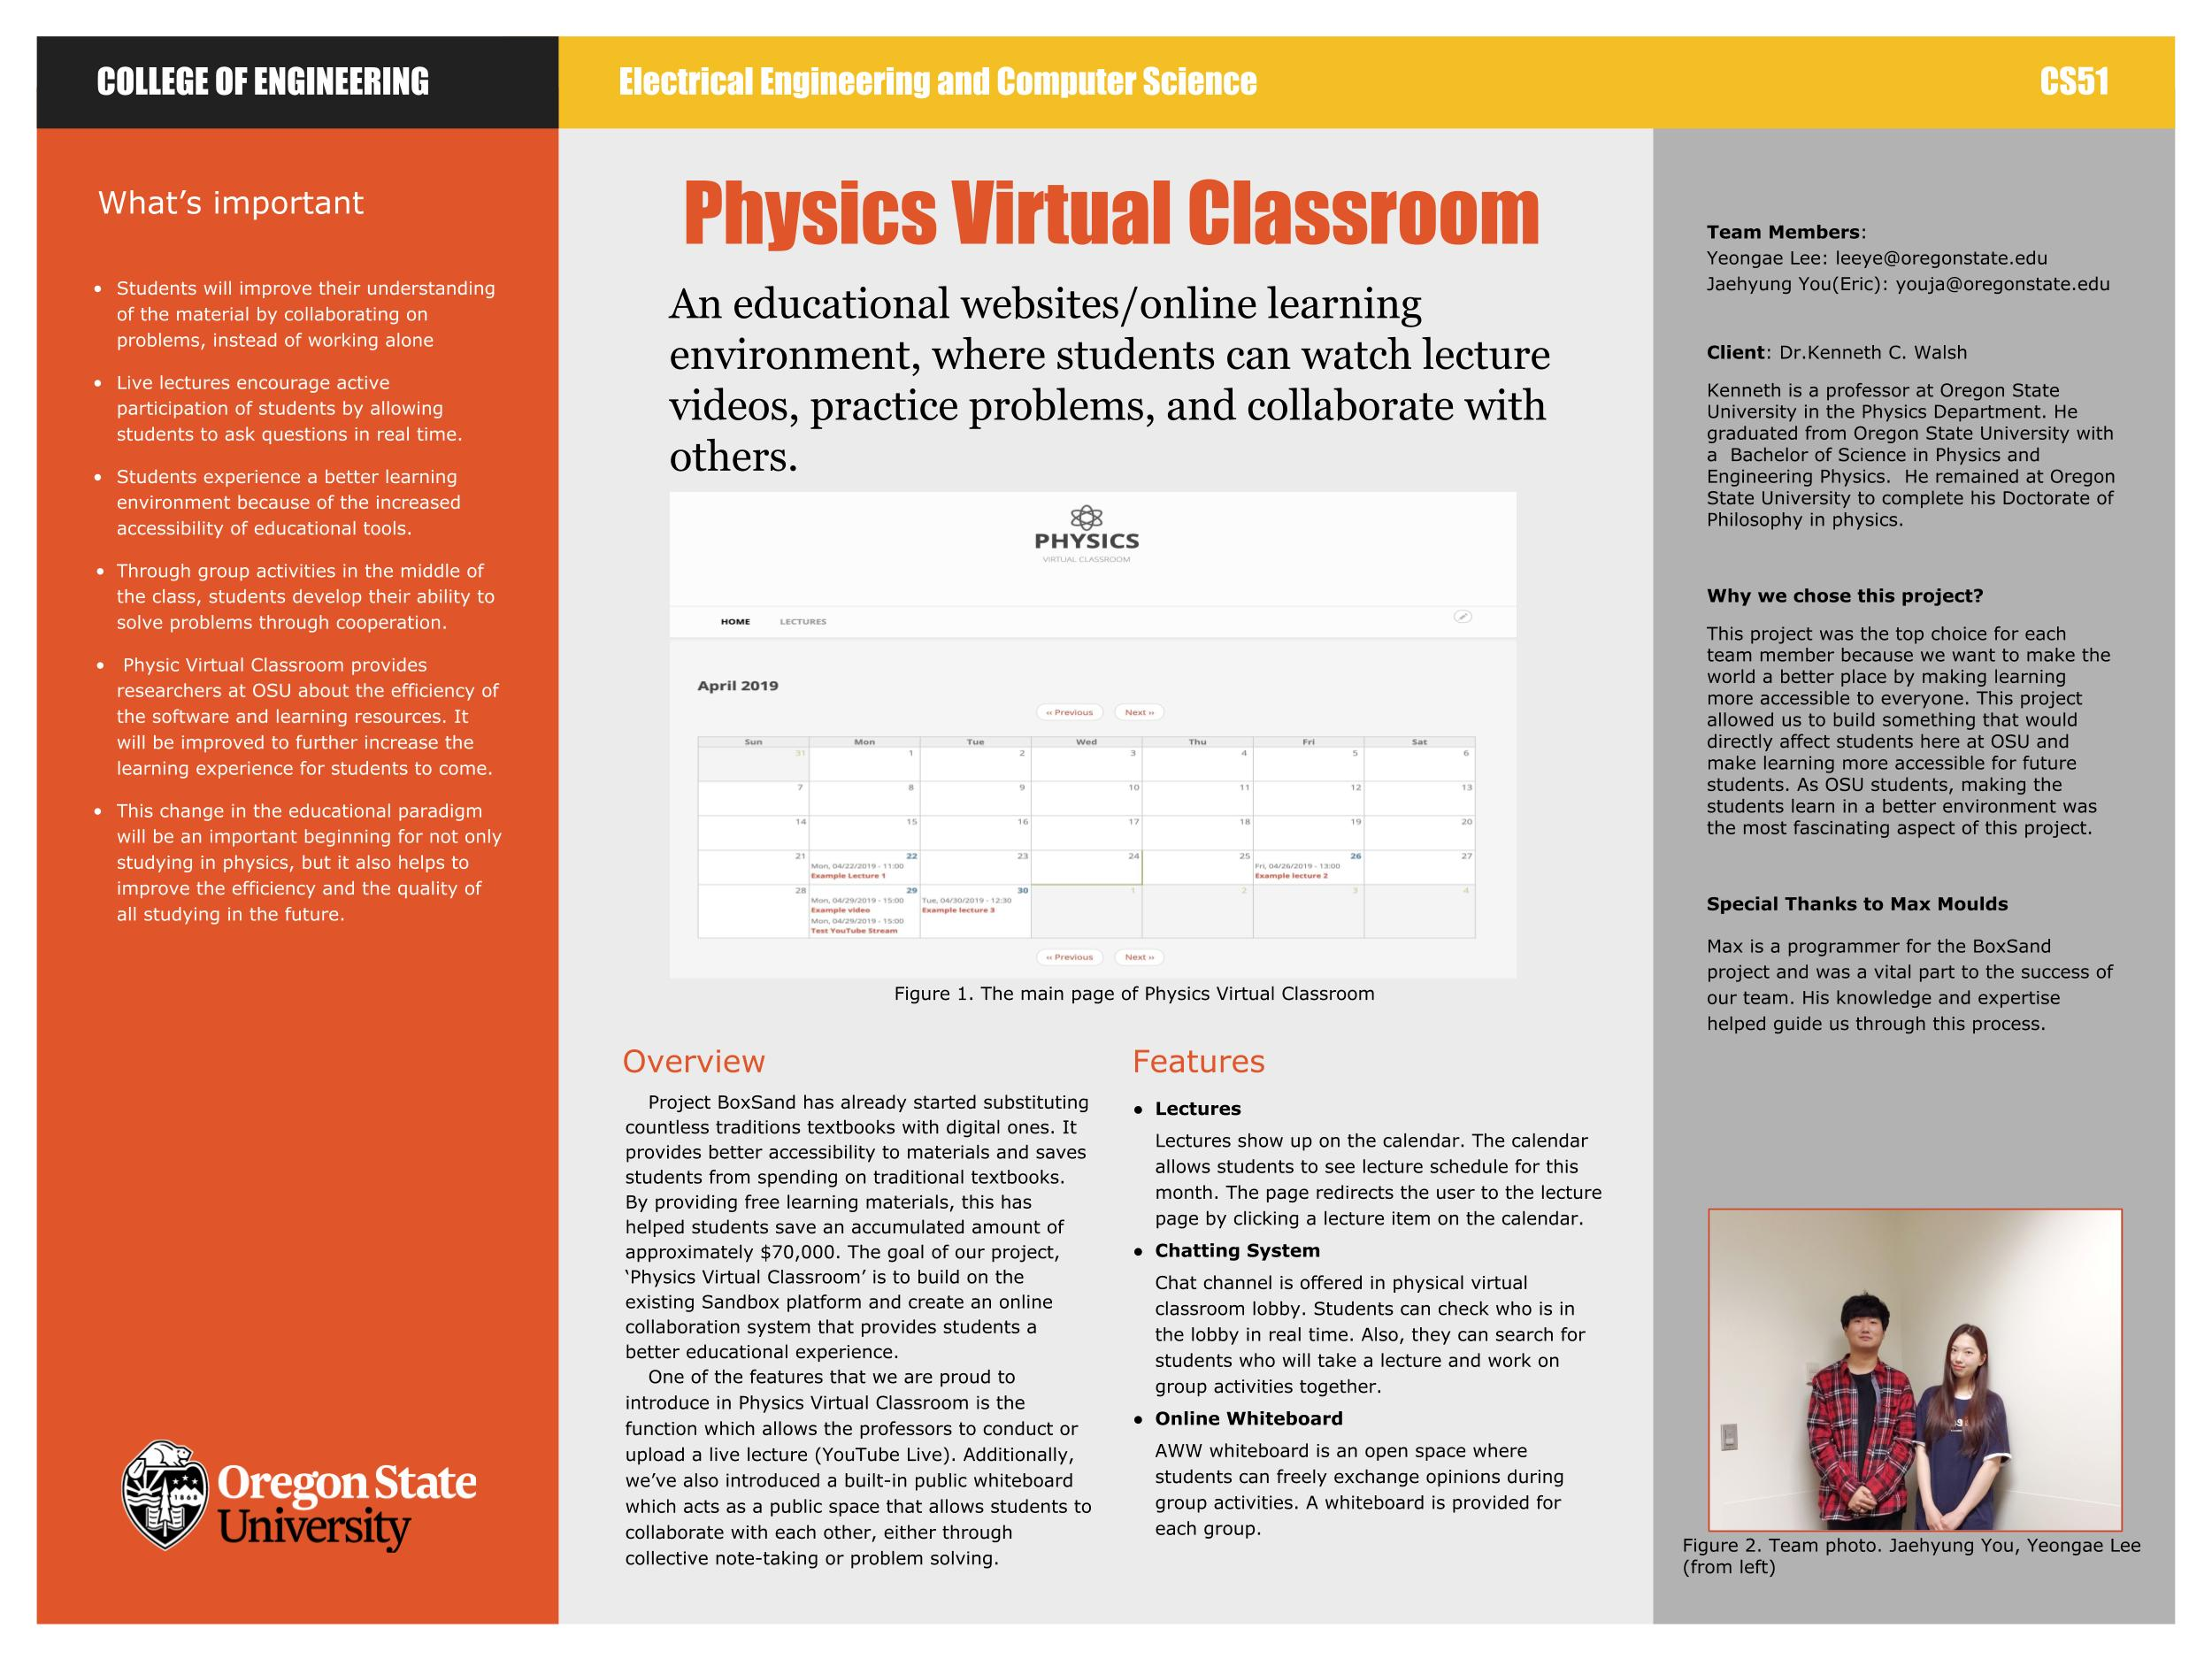
\includegraphics[width=1.0\textwidth]{Final_Poster/group51_AsyncSync_expo_poster_final}
        \caption{Expo Poster}
    \end{figure}

\clearpage
\section{Project Documentation}
    \subsection{Installation}
        \subsubsection{Prerequisite}
            You must be able to access the repository or the code. We are using Drupal8 as our developing environment. Any requirement will be installed if you follow the installation below. Any other requirement for using Drupal8, refer to the following link: https://www.drupal.org/docs/8/system-requirements

            \medskip \medskip \medskip
            \textbf{Note (You have to read this note before doing further actions):}
            \begin{itemize}
                \item The whole code for the current project is under "html" folder.
                \item You must use 'sqlbackup.sql' database file for completing to build the whole website.
                \item Documents folder is for all the documentation of the project.
                \item ph-virtual-classroom is the code we worked on. Now, we don't use the code anymore.
                \item The code in this repository only gives you make a simple drupal website. (in 'html' folder)
                \item The site can't do any functions without the current server-database. (`sqlbackup.sql.zip')
            \end{itemize}

        \subsubsection{Basic Program Installation: Drupal and MAMP}
            You may need to download Drupal8 (if the method I introduce below doesn't work) Drupal8 Download Clone git repository first. Please follow the following instructions (YouTube videos). You don't need to download Drupal from the Drupal website. You will use the  `html' folder as Drupal installer in this repository.
                \begin{itemize}
                    \item Install Drupal on MacOS: https://www.youtube.com/watch?v=pOBArJn-tSQ
                    \item Install Drupal on Ubuntu18.04: https://www.youtube.com/watch?v=9SEpG0rOs1w
                    \item Install Drupal on Windows: https://www.youtube.com/watch?v=4Gl9s40vldY
                \end{itemize}
            Our current server is running on Ubuntu. This guide does not include the guide for Linux users, so you may need to know how you can access `MyphpAdmin’ (We need this later) in your own Linux. \\
            \textbf{For Windows and MacOS users need to download `MAMP’ application to run the server. Download MAMP: https://www.mamp.info/en/downloads/}

        \subsubsection{Install Drupal and import Database on your local machine}
            \begin{enumerate}
                \item Download MAMP and run MAMP. Then, you should see this program. Then, Click the `Start Servers’. The server is starting now.

                    \begin{figure}[!ht]
                        \centering
                        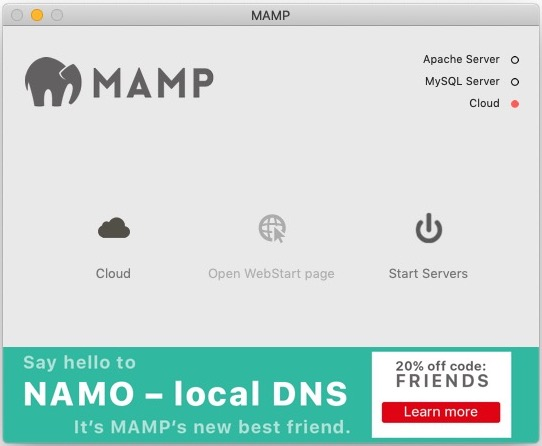
\includegraphics[width=0.35\textwidth]{Project_Document/MAMP}
                        \caption{MAMP Application}
                    \end{figure}
\newpage
                \item Now you can see this page, then your MAMP application works.

                    \begin{figure}[!ht]
                        \centering
                        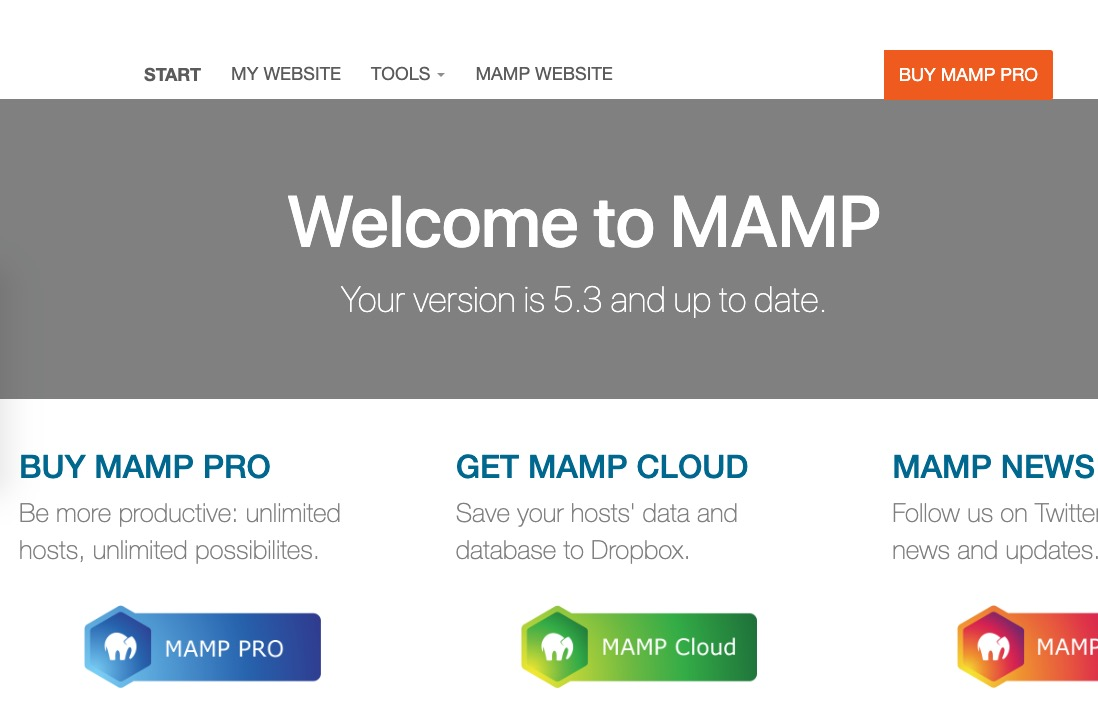
\includegraphics[width=0.55\textwidth]{Project_Document/setup}
                        \caption{MAMP Page}
                    \end{figure}

                \item Now, you need to find the folder that will render your code to its server.

                    \begin{itemize}
                        \item For MacOS, move`html' from this repository to `/Application/MAMP/htdocs' (if you are using MAMP).
                        \item For Windows, move `html' from this repository to `Local Disk/MAMP/htdocs' (if you are using MAMP), and keep following the instruction for MacOS.
                        \item (if) For Ubuntu, locate to the folder `html' in /var/www/ (if you followed the instruction the above).
                    \end{itemize}

                    \begin{figure}[!ht]
                           \centering
                           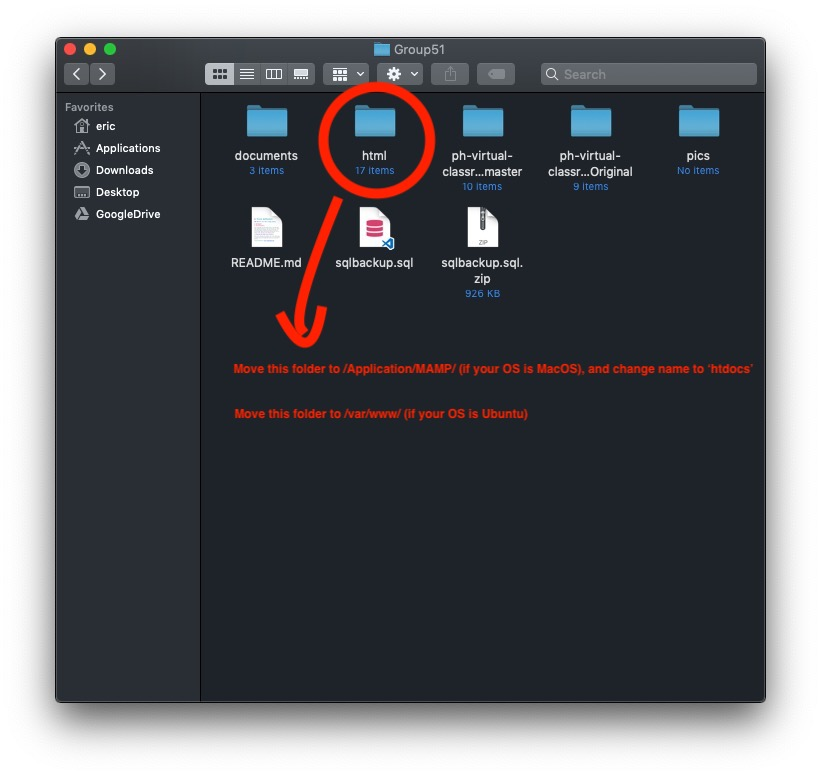
\includegraphics[width=0.7\textwidth]{Project_Document/macos}
                        \caption{Project File Folder}
                    \end{figure}
\newpage
                \item You need to go to your `PHPMYADMIN’. This is where you can find `phpMyAdmin' by using MAMP (Click `TOOLS' in the banner, then click `PHPMYADMIN')

                    \begin{figure}[!ht]
                           \centering
                             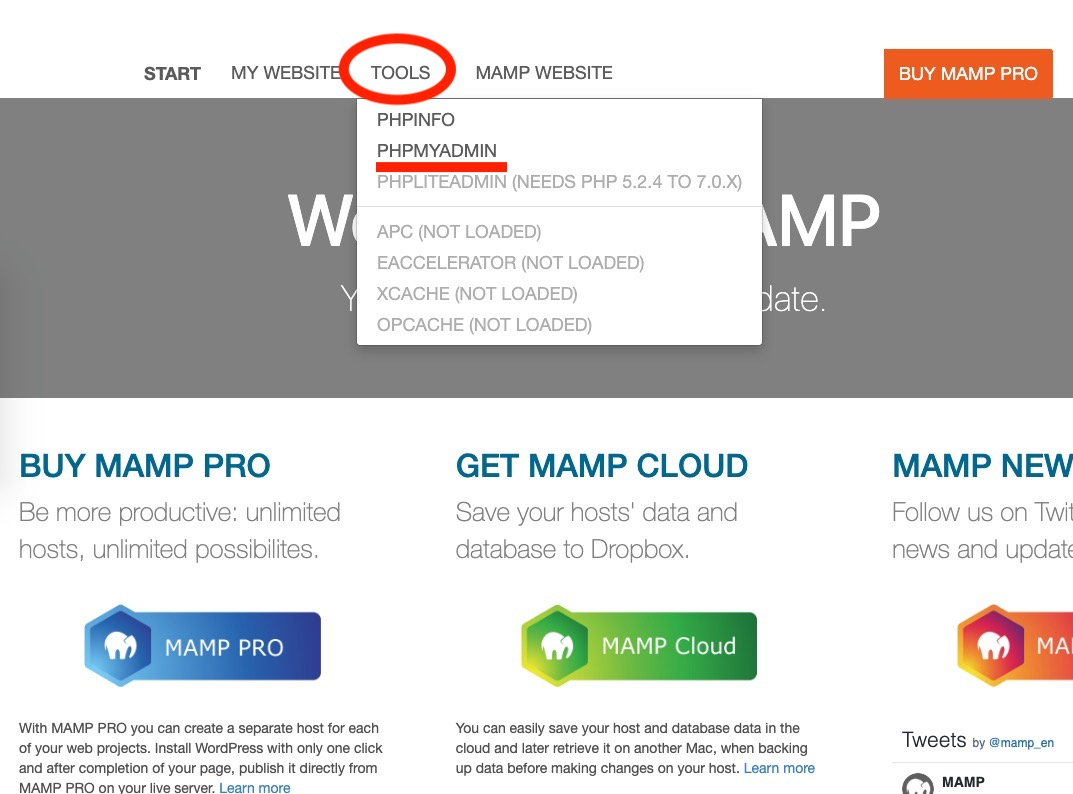
\includegraphics[width=0.7\textwidth]{Project_Document/phpmyadmin}
                        \caption{phpMyAdmin on MAMP}
                    \end{figure}

                \item Now, you need to open `phpMyAdmin' and create a database. (I named it drupal)

                    \begin{figure}[!ht]
                           \centering
                           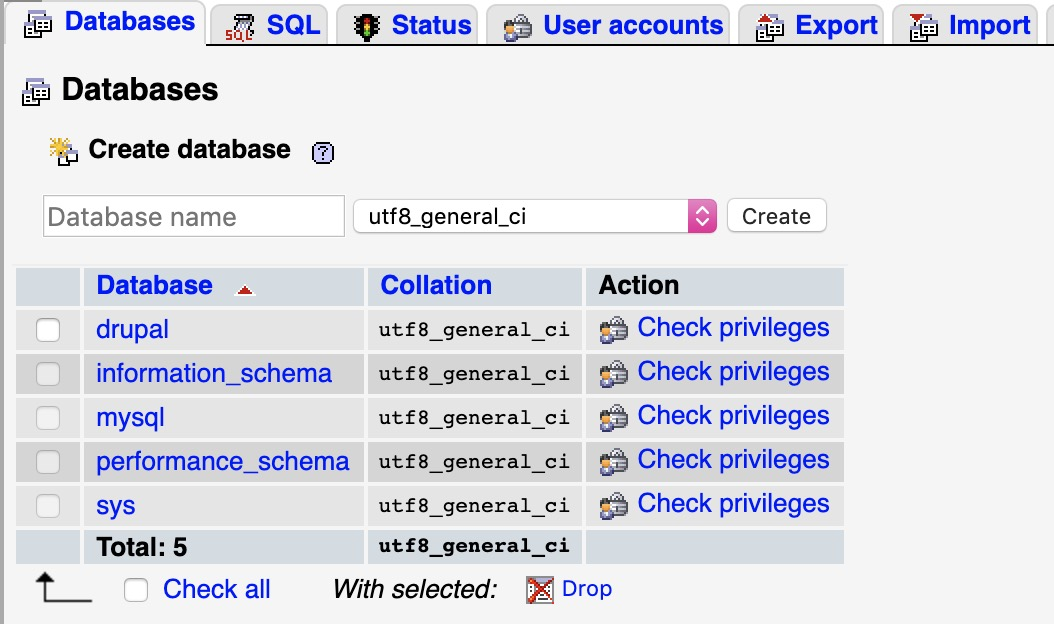
\includegraphics[width=0.7\textwidth]{Project_Document/1}
                        \caption{phpMyAdmin}
                    \end{figure}
\newpage
                \item Then, click the database and go to `Import' tab at the top. (I marked in the red square)

                    \begin{figure}[!ht]
                           \centering
                           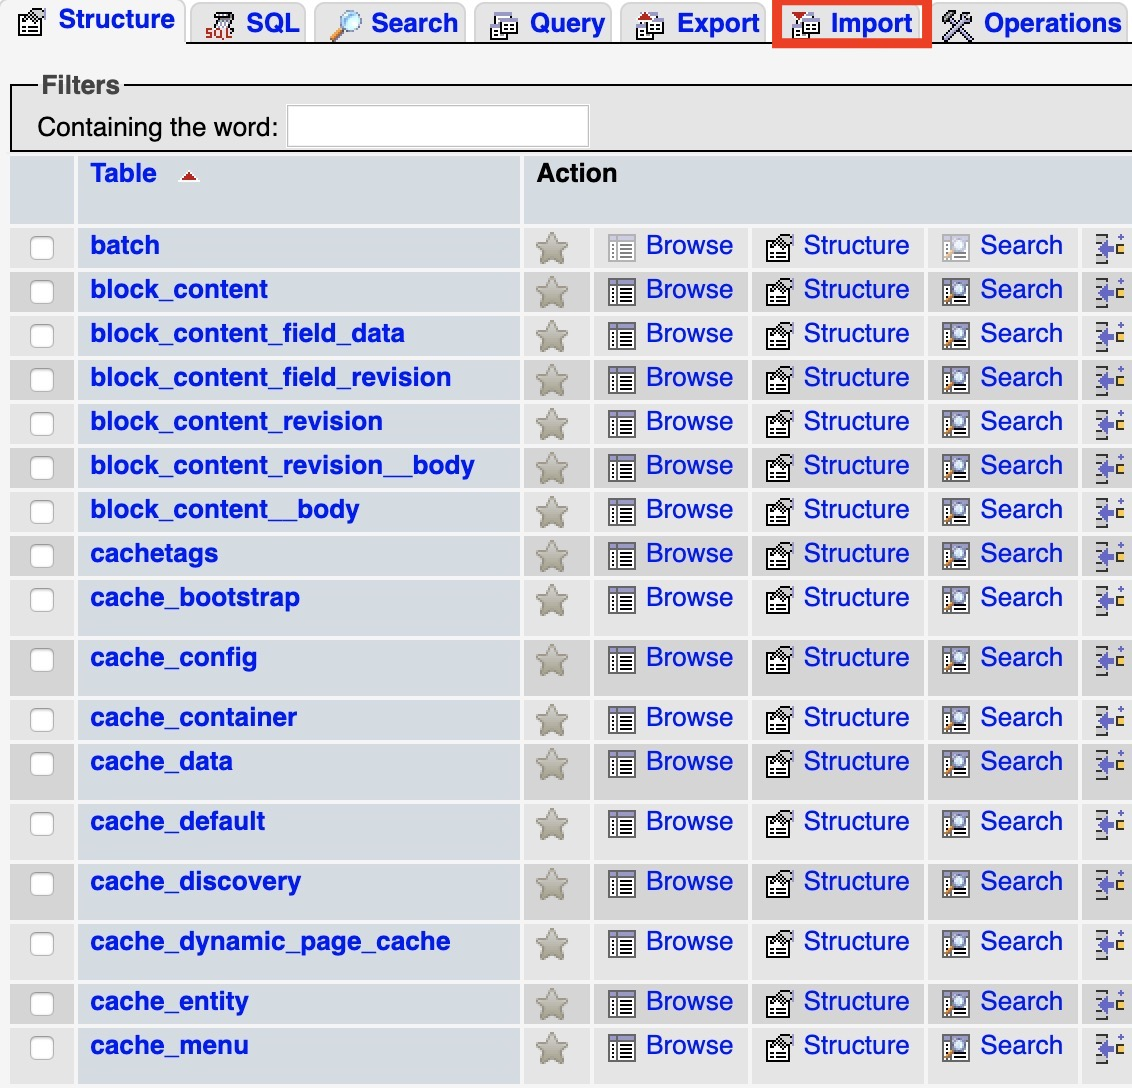
\includegraphics[width=0.7\textwidth]{Project_Document/2}
                        \caption{`Import' Button on phpMyAdmin }
                    \end{figure}

                \item Then, click the `choose the file' and open the file name `sqlbackup.sql.zip' in thie repo. Now, you have imported our back-up files from the server. \\
                Open this file by any test editor

\begin{lstlisting}[language=bash]
`html' or `any folder for your Drupal directory'/sites/default/settings.php
\end{lstlisting}

                Find this lines of the code (it is located at the very bottom) \\

                    \begin{figure}[!ht]
                           \centering
                           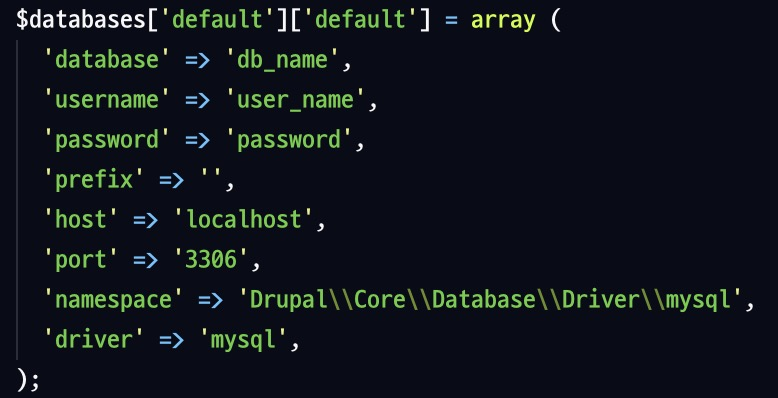
\includegraphics[width=0.5\textwidth]{Project_Document/codes}
                        \caption{Database Code}
                    \end{figure}

                Please change database, username and password sections to match your local settings (the database you have imported the above) Finally, you can connect our Drupal Website. If you are using MAMP, MAMP already sets the username and the password for MySQL for you. This is where you can find your username and password (in MAMP main page). All you needs are user and password. (Mostly, these are already set as root and root)

                    \begin{figure}[!ht]
                           \centering
                           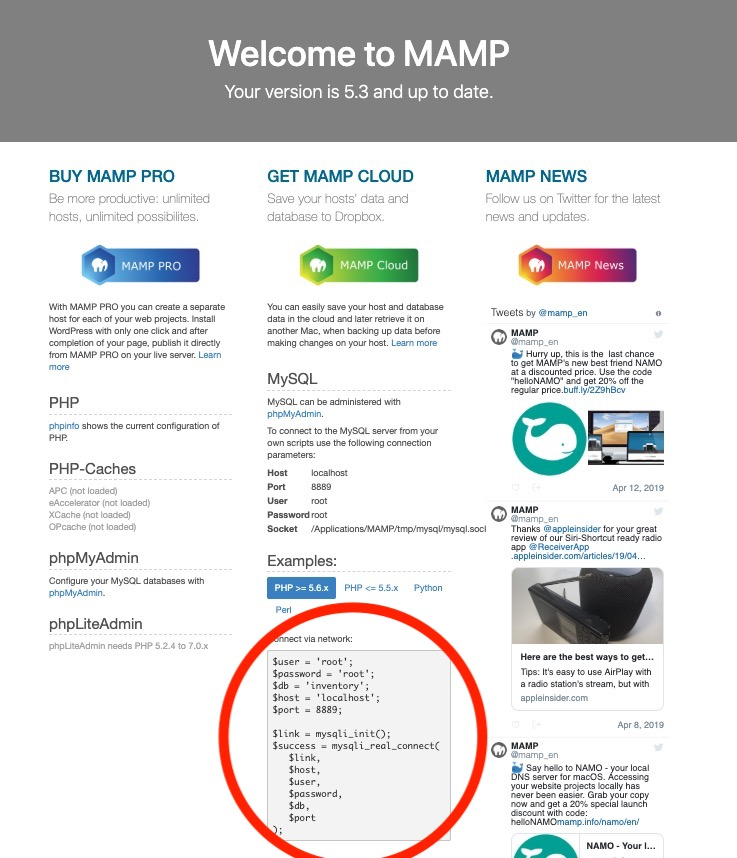
\includegraphics[width=0.5\textwidth]{Project_Document/sqlinfo}
                        \caption{Database Information on MAMP}
                    \end{figure}

            \item You can connect to your localhost by:

\begin{lstlisting}[language=bash]
http://localhost or http://localhost:8888
\end{lstlisting}

            You may want to log in to the site to see how the site actually works. (Click `+' sign at the top right corner)

                \begin{figure}[!ht]
                       \centering
                         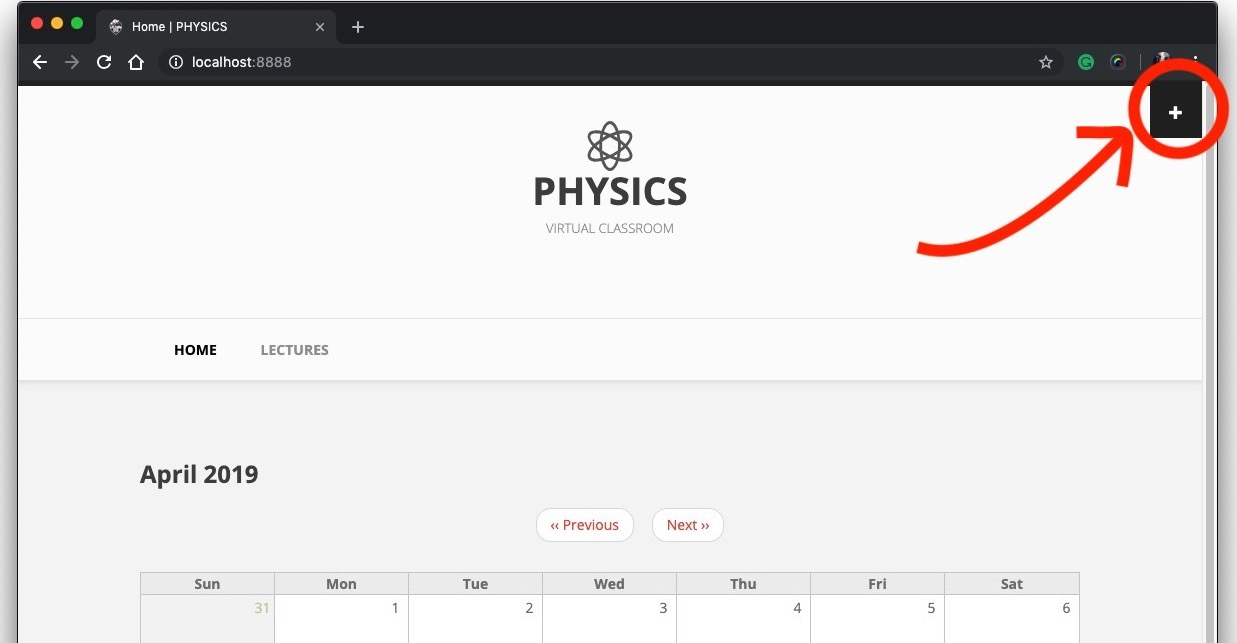
\includegraphics[width=0.6\textwidth]{Project_Document/login.jpg}
                    \caption{Login Button on Physic Virtual Classroom Website}
                \end{figure}
\newpage
            If you don’t know the username and the password, please contact Walsh, Kenneth.

            Note: if you are trying to connect to Drupal, not by localhost, you need to modify this code in the same setting.php file. Add your host name in the array.

                \begin{figure}[!ht]
                       \centering
                       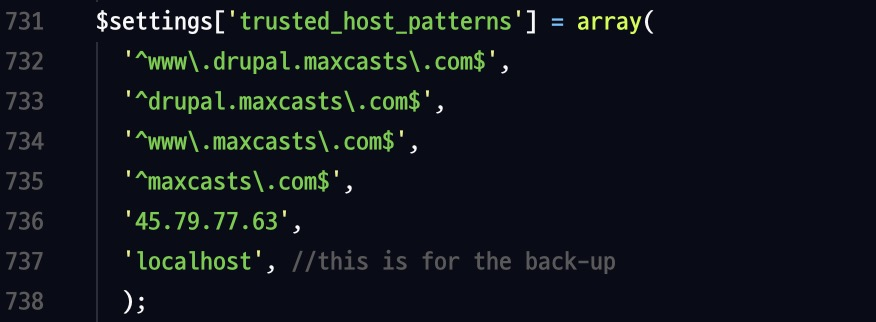
\includegraphics[width=0.7\textwidth]{Project_Document/host.jpg}
                    \caption{setting.php File}
                \end{figure}
        \end{enumerate}

    \subsection{User manual}
        \subsubsection{Add Lecture}
            \begin{enumerate}
            	\item Log in to an administrator account. Only users who have an administration account can add lectures.
            	\item Click `Content' on the toolbar.
            	   \begin{figure}[!ht]
            	        \centering
                        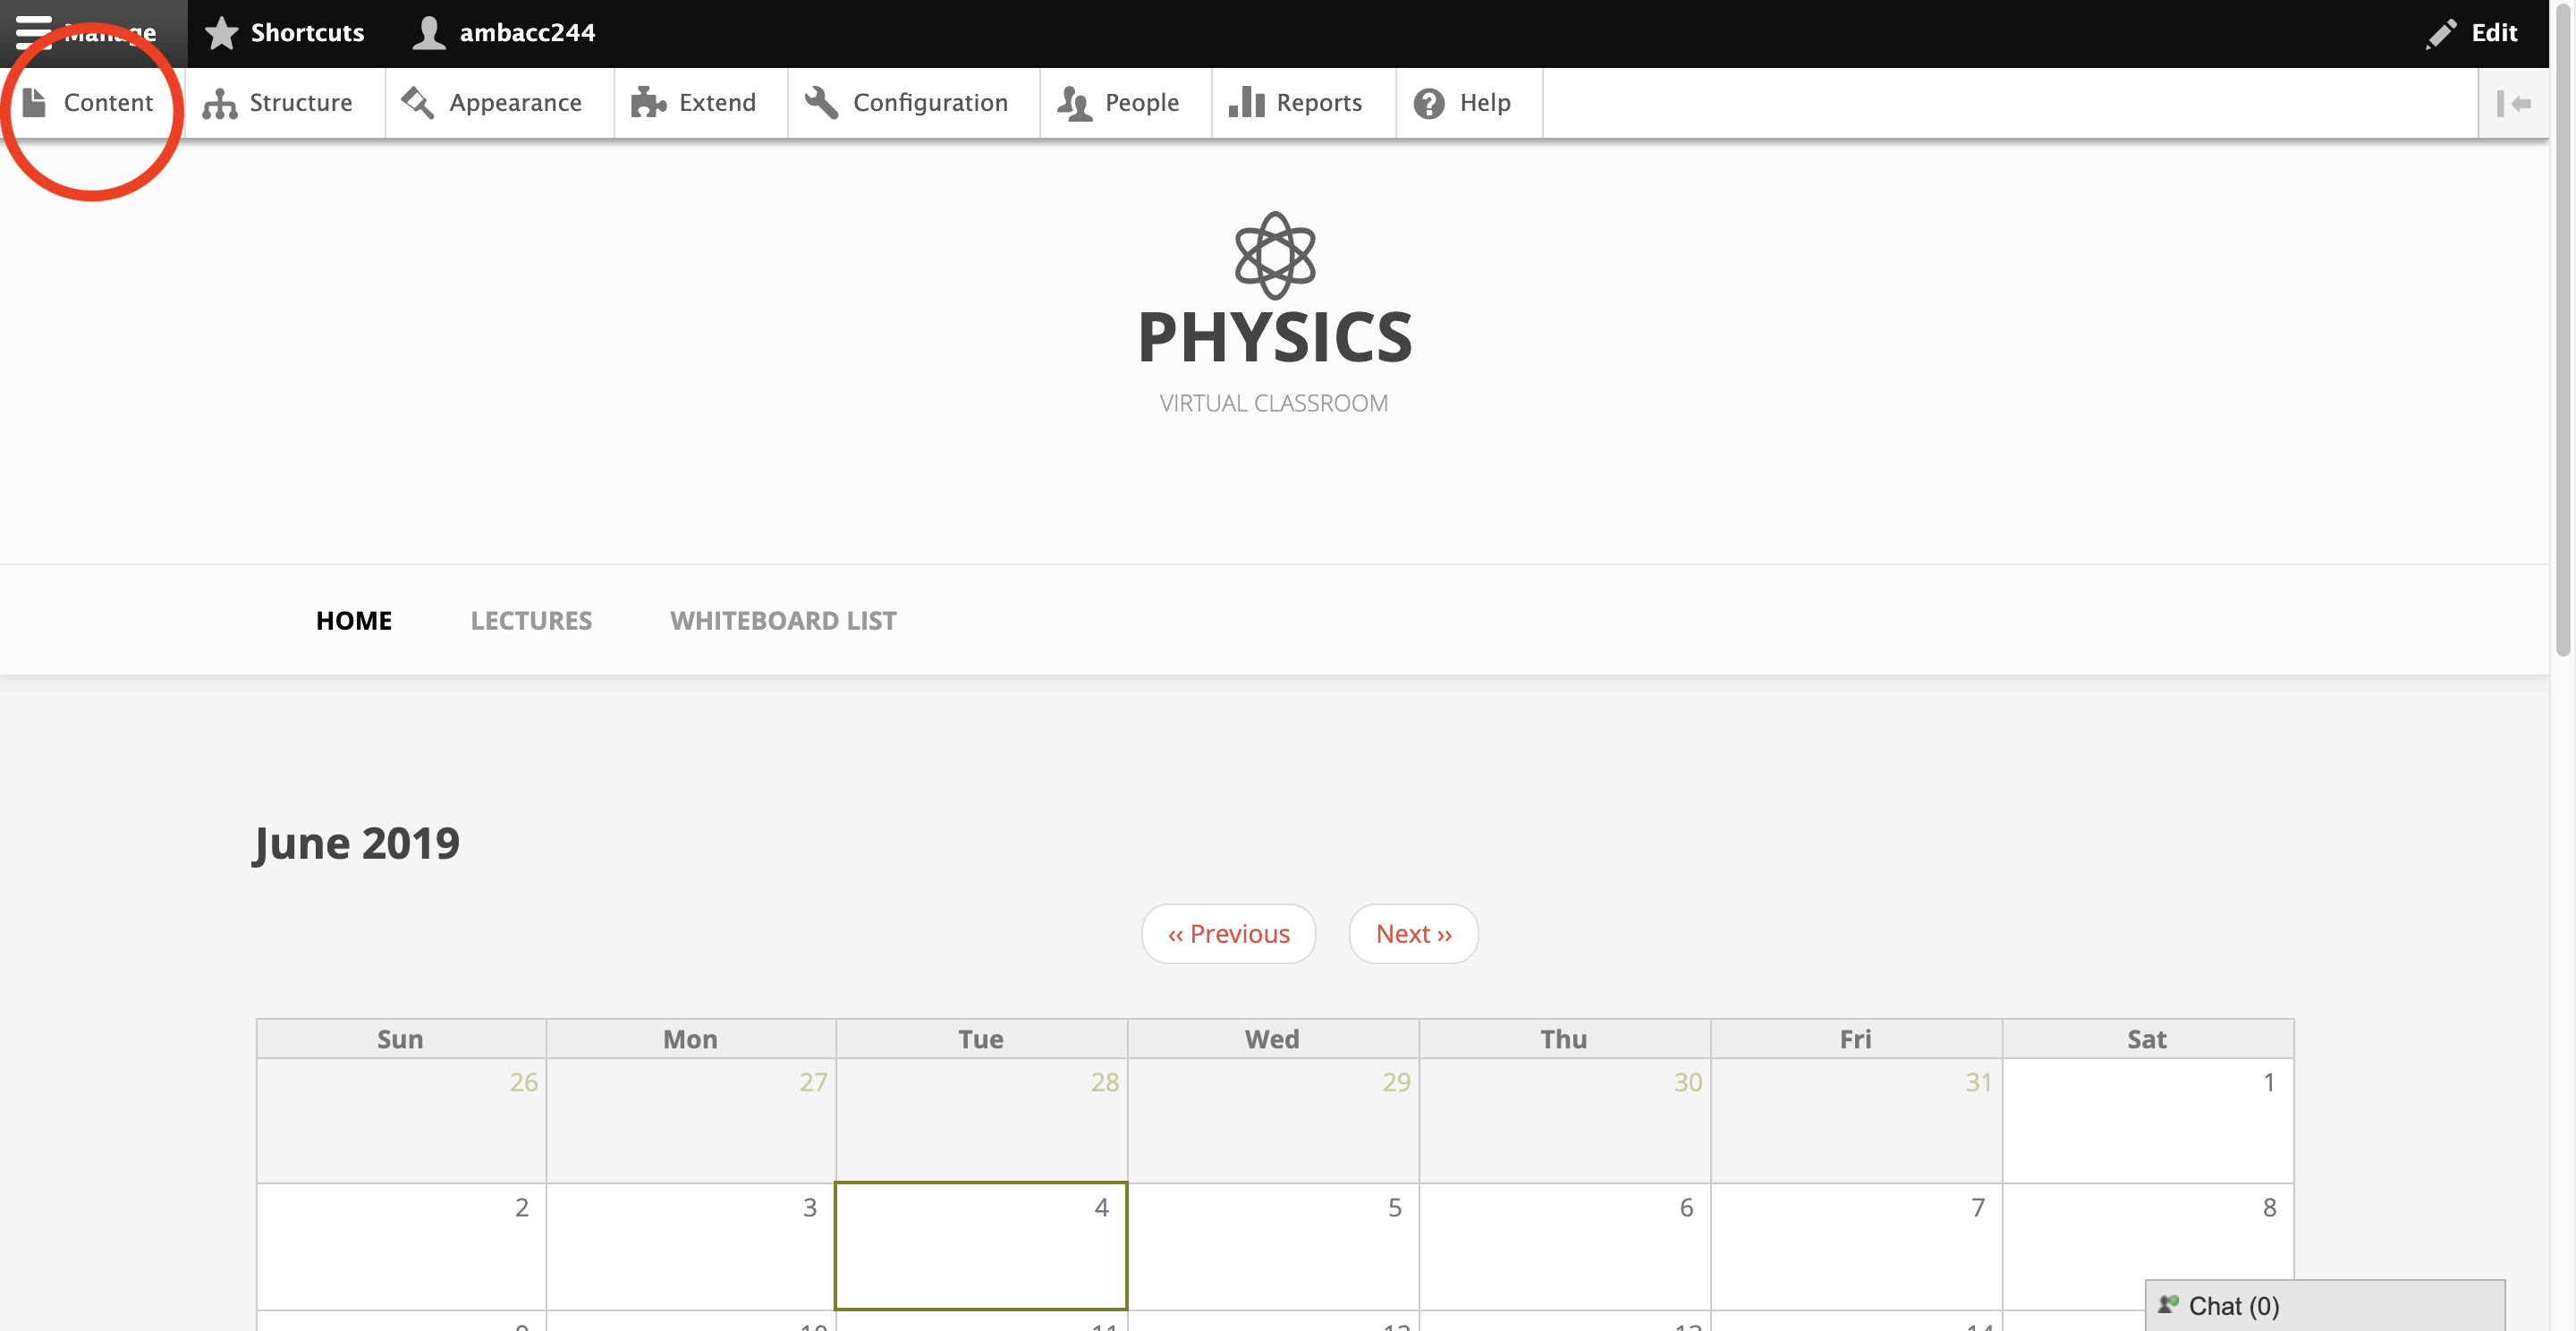
\includegraphics[width=0.7\textwidth]{Project_Document/content}
                        \caption{`Content' Button on the Physics Virtual Classroom Website}
                    \end{figure}
            	\item Click `+Add content' $\,\to\,$ `Lecture Video'
            	\item Need to fill out `Create Lecture Video' form. There are four parts to fill out which are title, body, date, and video
            	    \begin{itemize}
                    	\item Title: title of the lecture
                    	\item Body: lecture description
                    	\item Data: lecture date and time
                    	\item Video: YouTube or YouTube live video link
                    \end{itemize}
            	\item Click `Preview' to check lecture information again.
            	\item Click `Save' to add the lecture.
            \end{enumerate}

        \subsubsection{Edit or Delete Lecture}
            \begin{enumerate}
            	\item Log in to an administrator account. Only users who have an administration account can edit lectures.

            	\item Click `LECTURES' on the toolbar.
            	    \begin{figure}[!ht]
            	        \centering
                        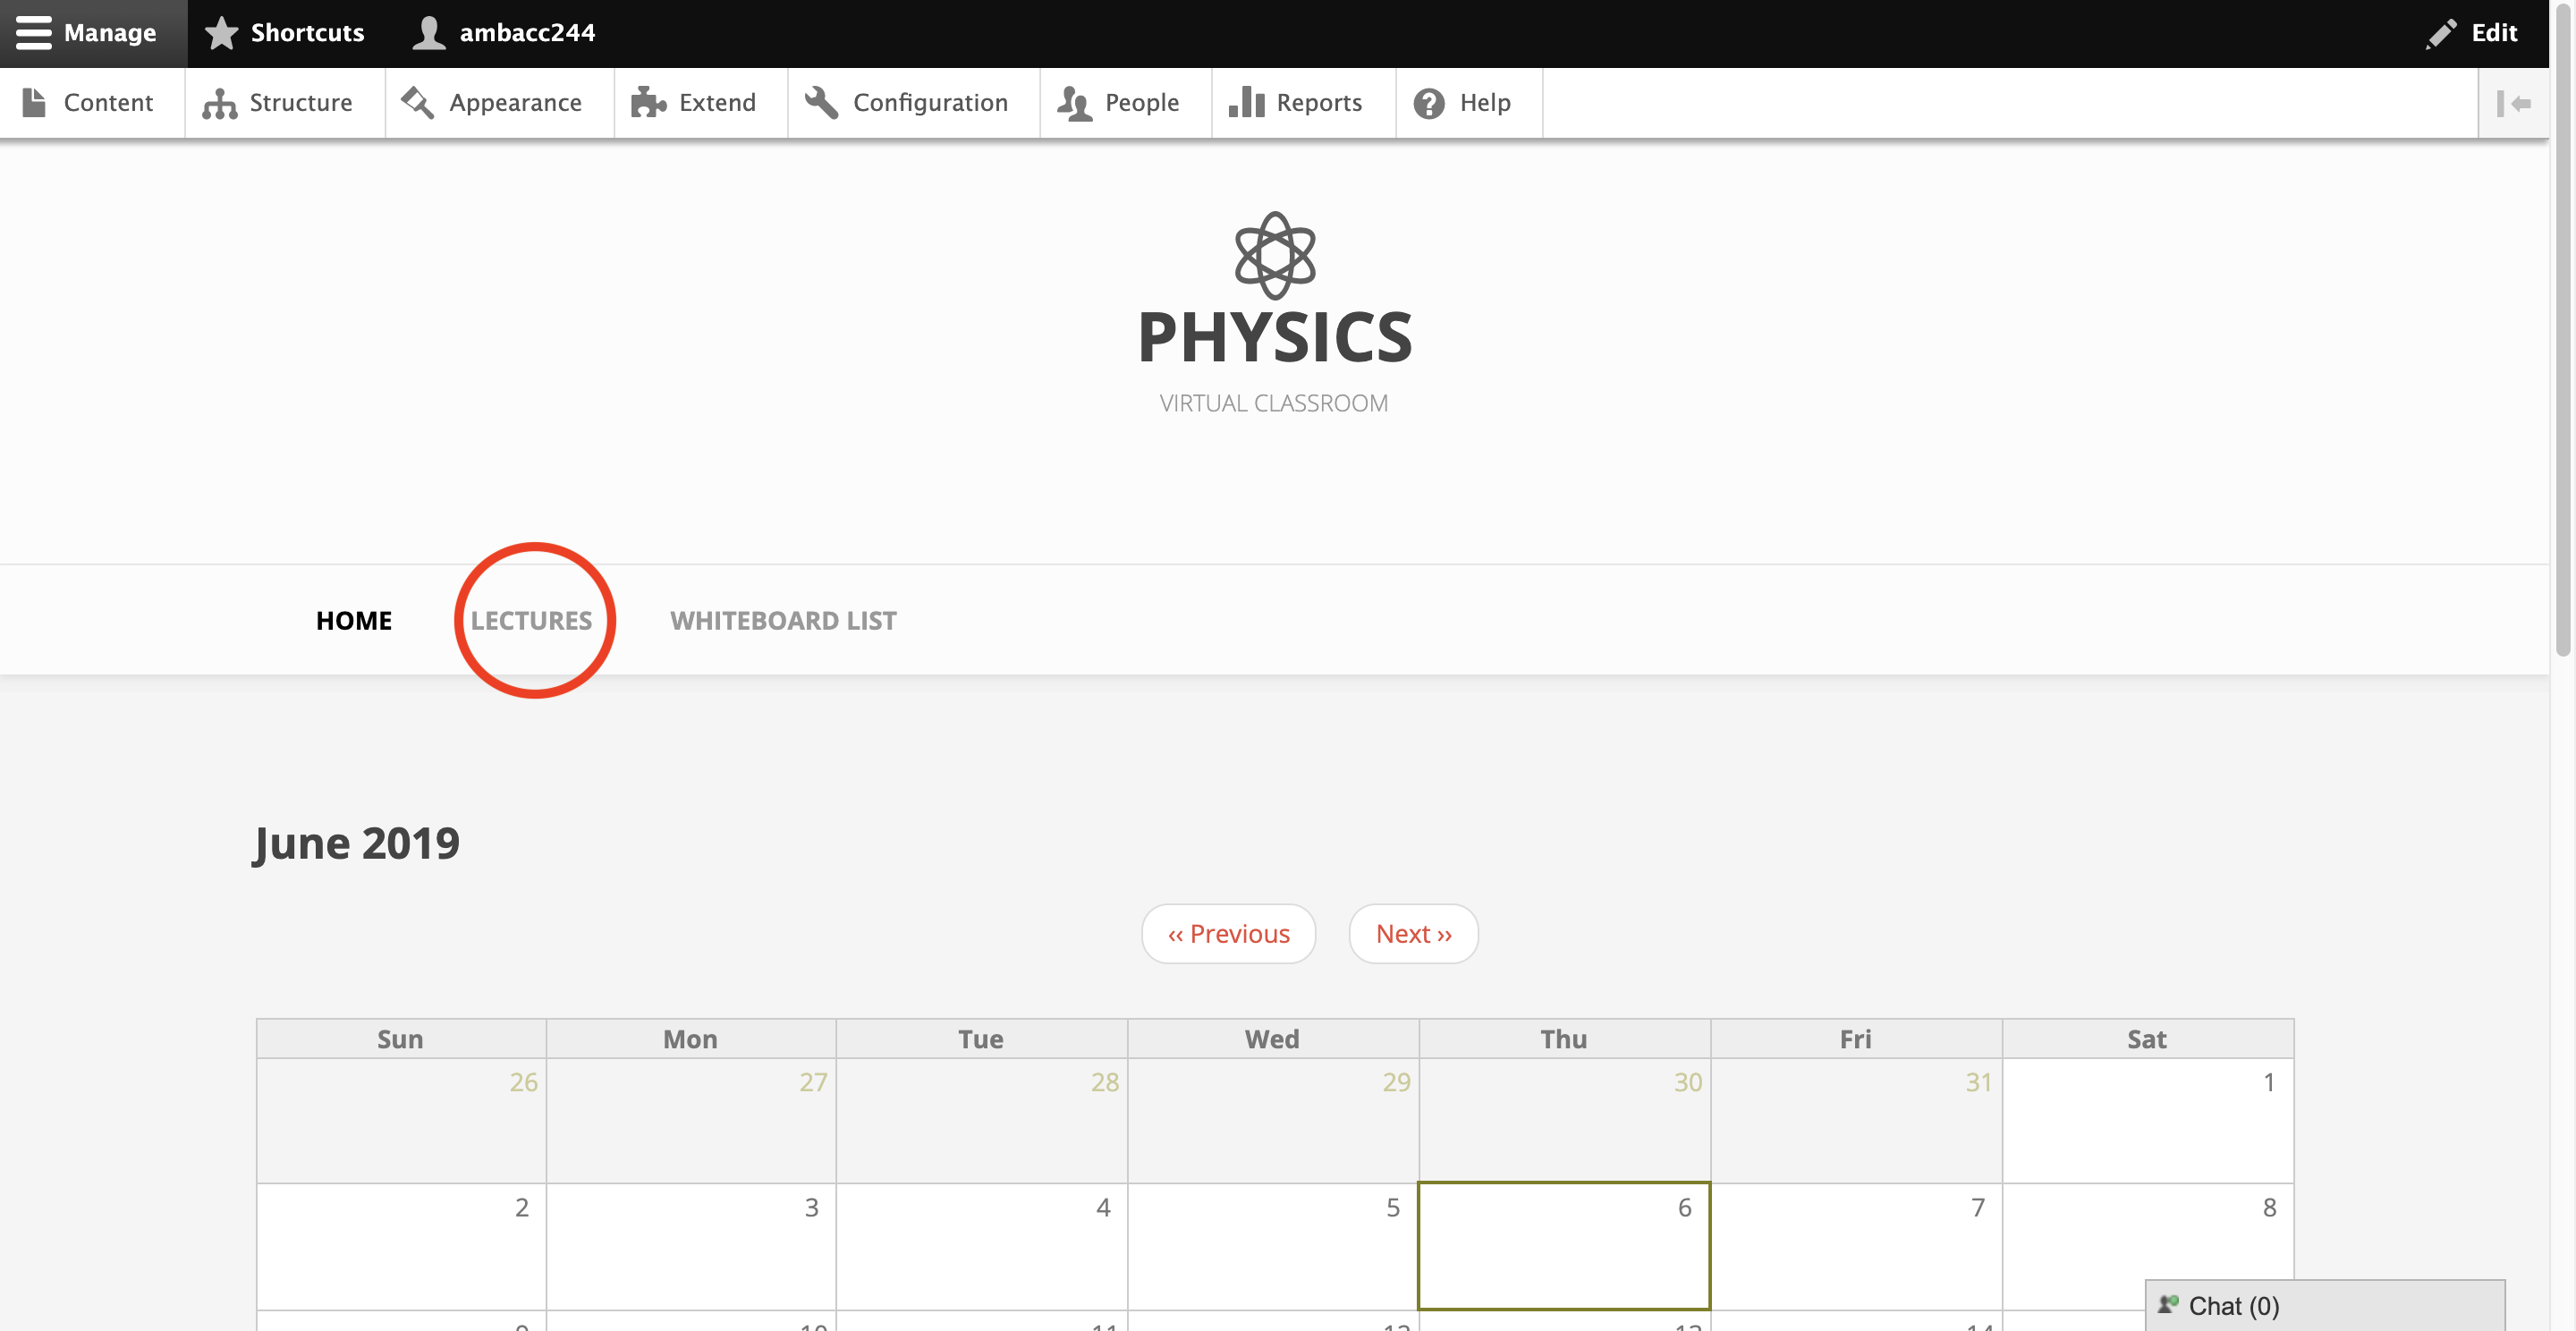
\includegraphics[width=0.7\textwidth]{Project_Document/lectures.png}
                        \caption{`LECTURES' Button on the Physics Virtual Classroom Website}
                    \end{figure}
            	\item Click the lecture which you want to edit or delete on the table.
            	\item Click `Edit' or `Delete' to edit or delete the lecture.
            \end{enumerate}

        \subsubsection{Add, Edit or Delete whiteboard on the whiteboard list}
            \begin{enumerate}
            	\item Log in to an administrator account. Only users who have an administration account can add lectures.
            	\item Click `WHITEBOARD LIST' on the toolbar.
            	    \begin{figure}[!ht]
            	        \centering
                        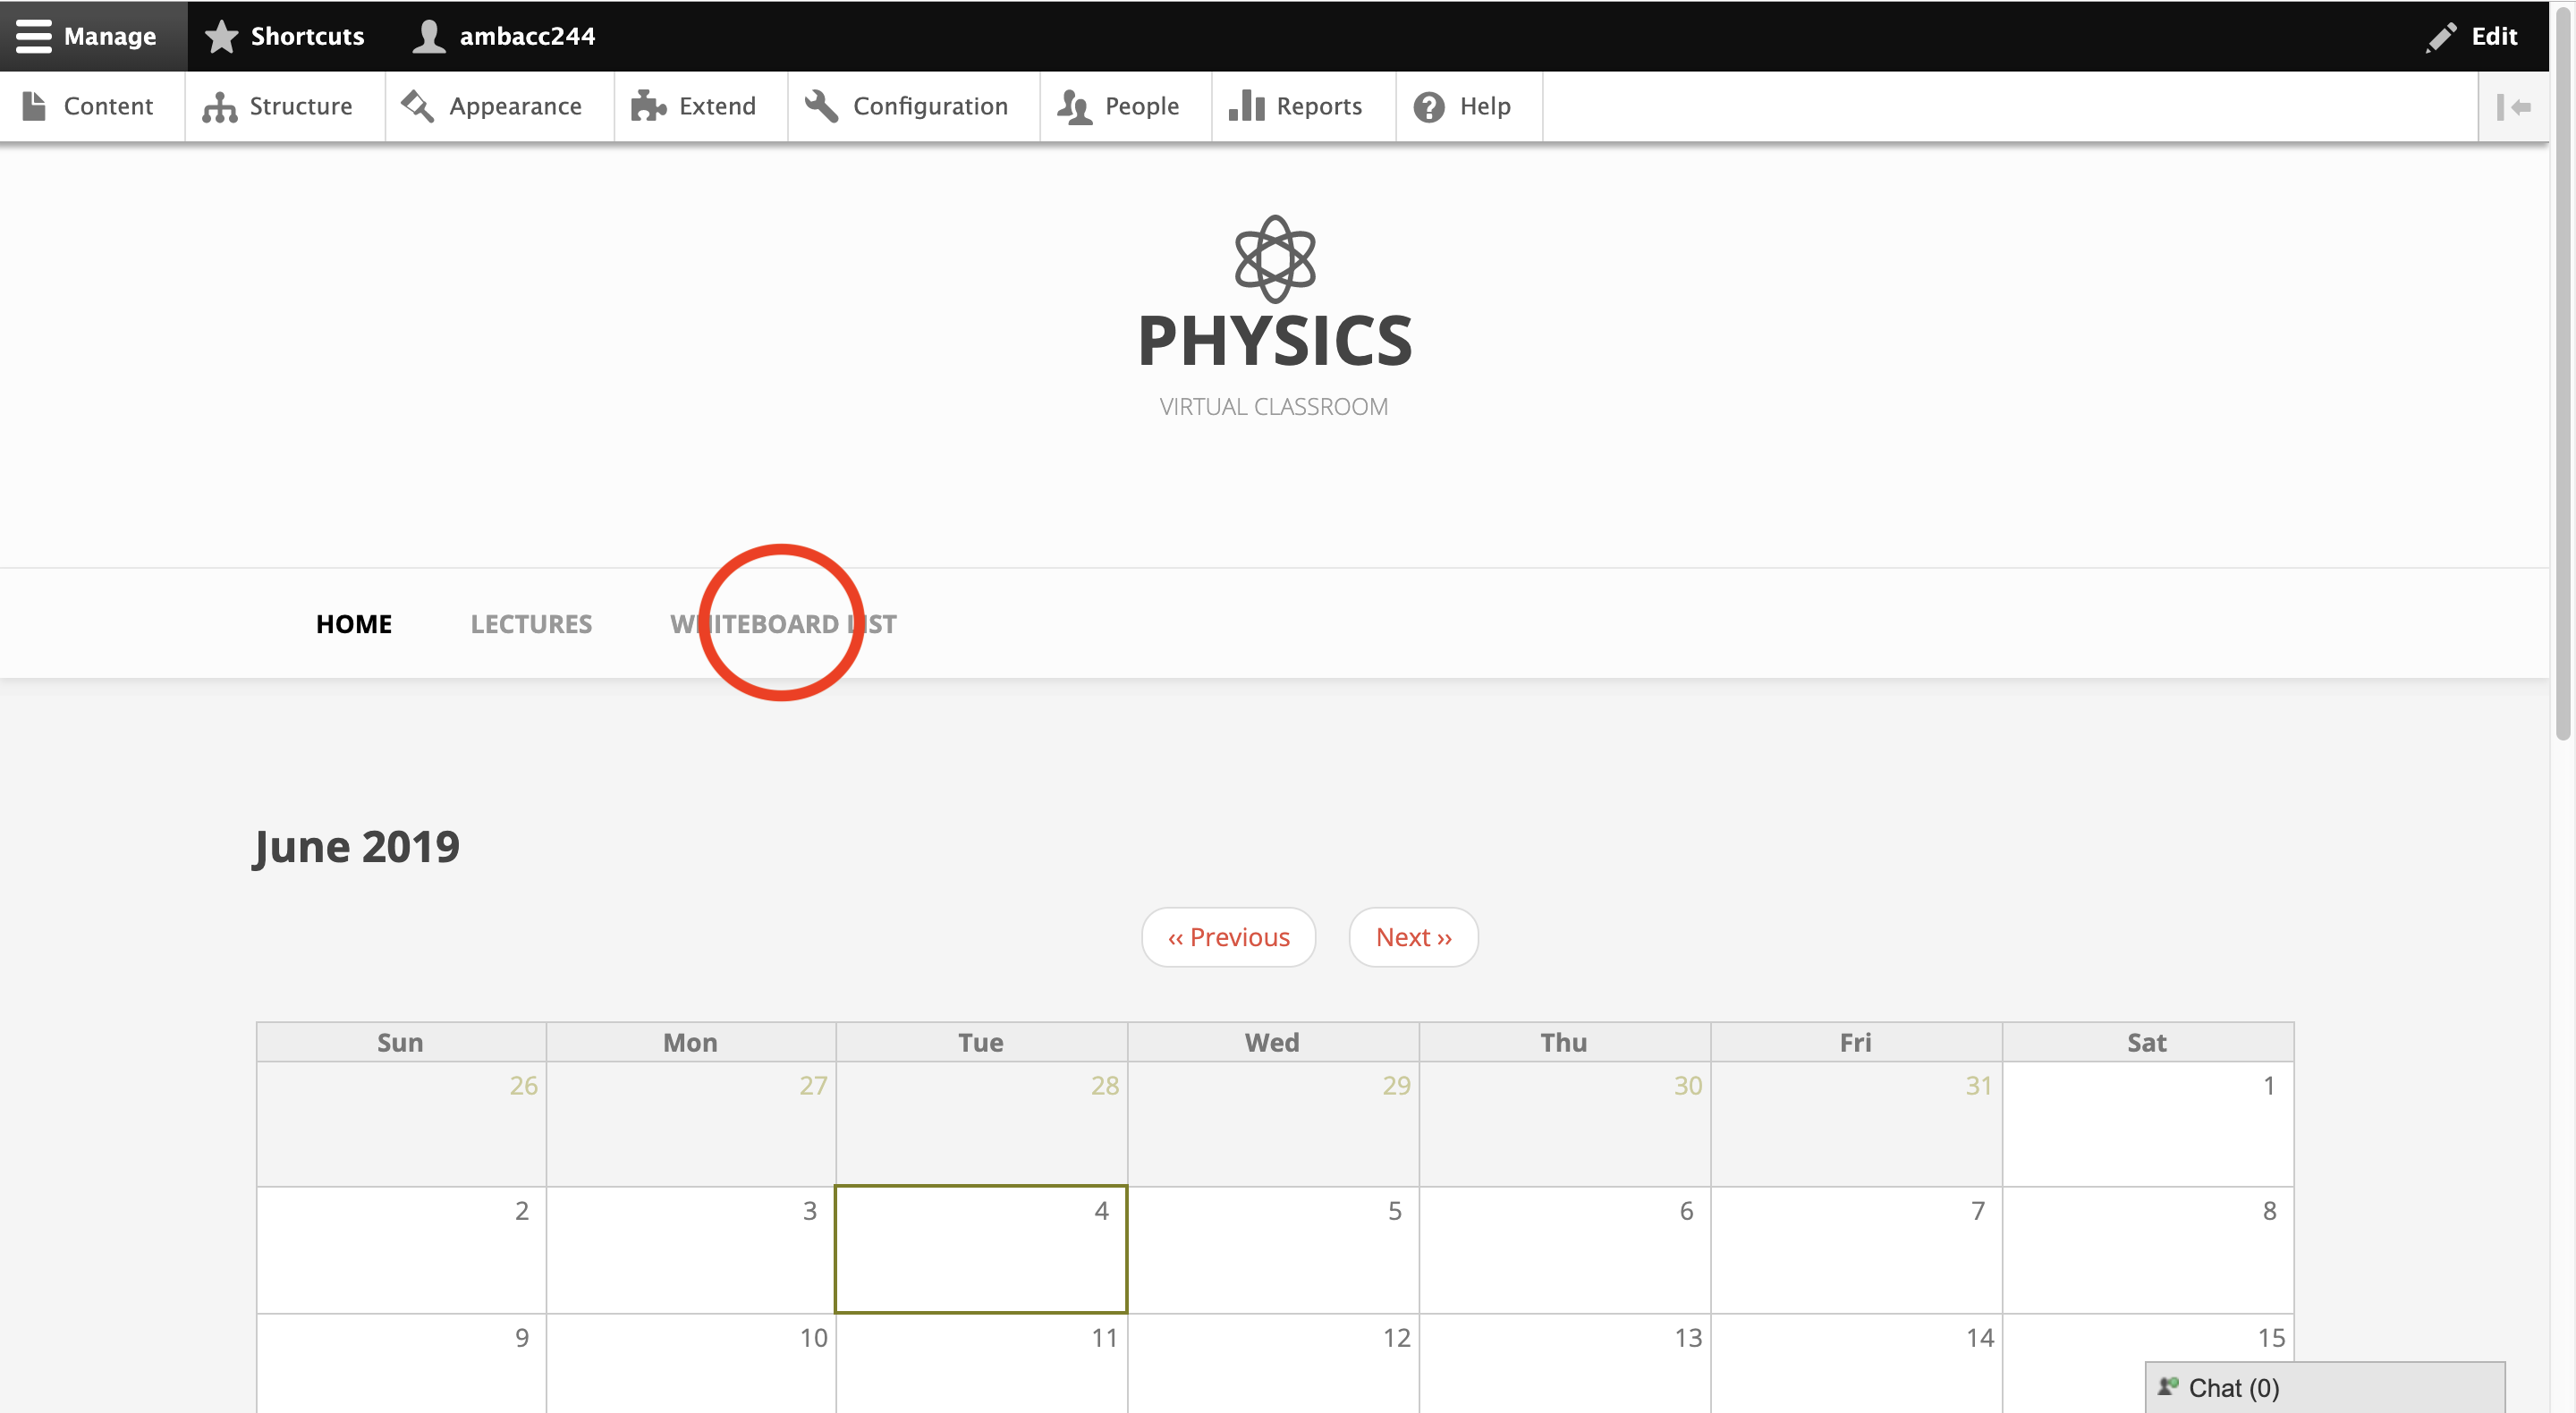
\includegraphics[width=0.7\textwidth]{Project_Document/whiteboard.png}
                        \caption{`WHITEBOARD LIST' Button on the Physics Virtual Classroom Website}
                    \end{figure}
\newpage
            	\item Click `Edit' $\,\to\,$ `Source'
            	    \begin{figure}[!ht]
            	        \centering
                        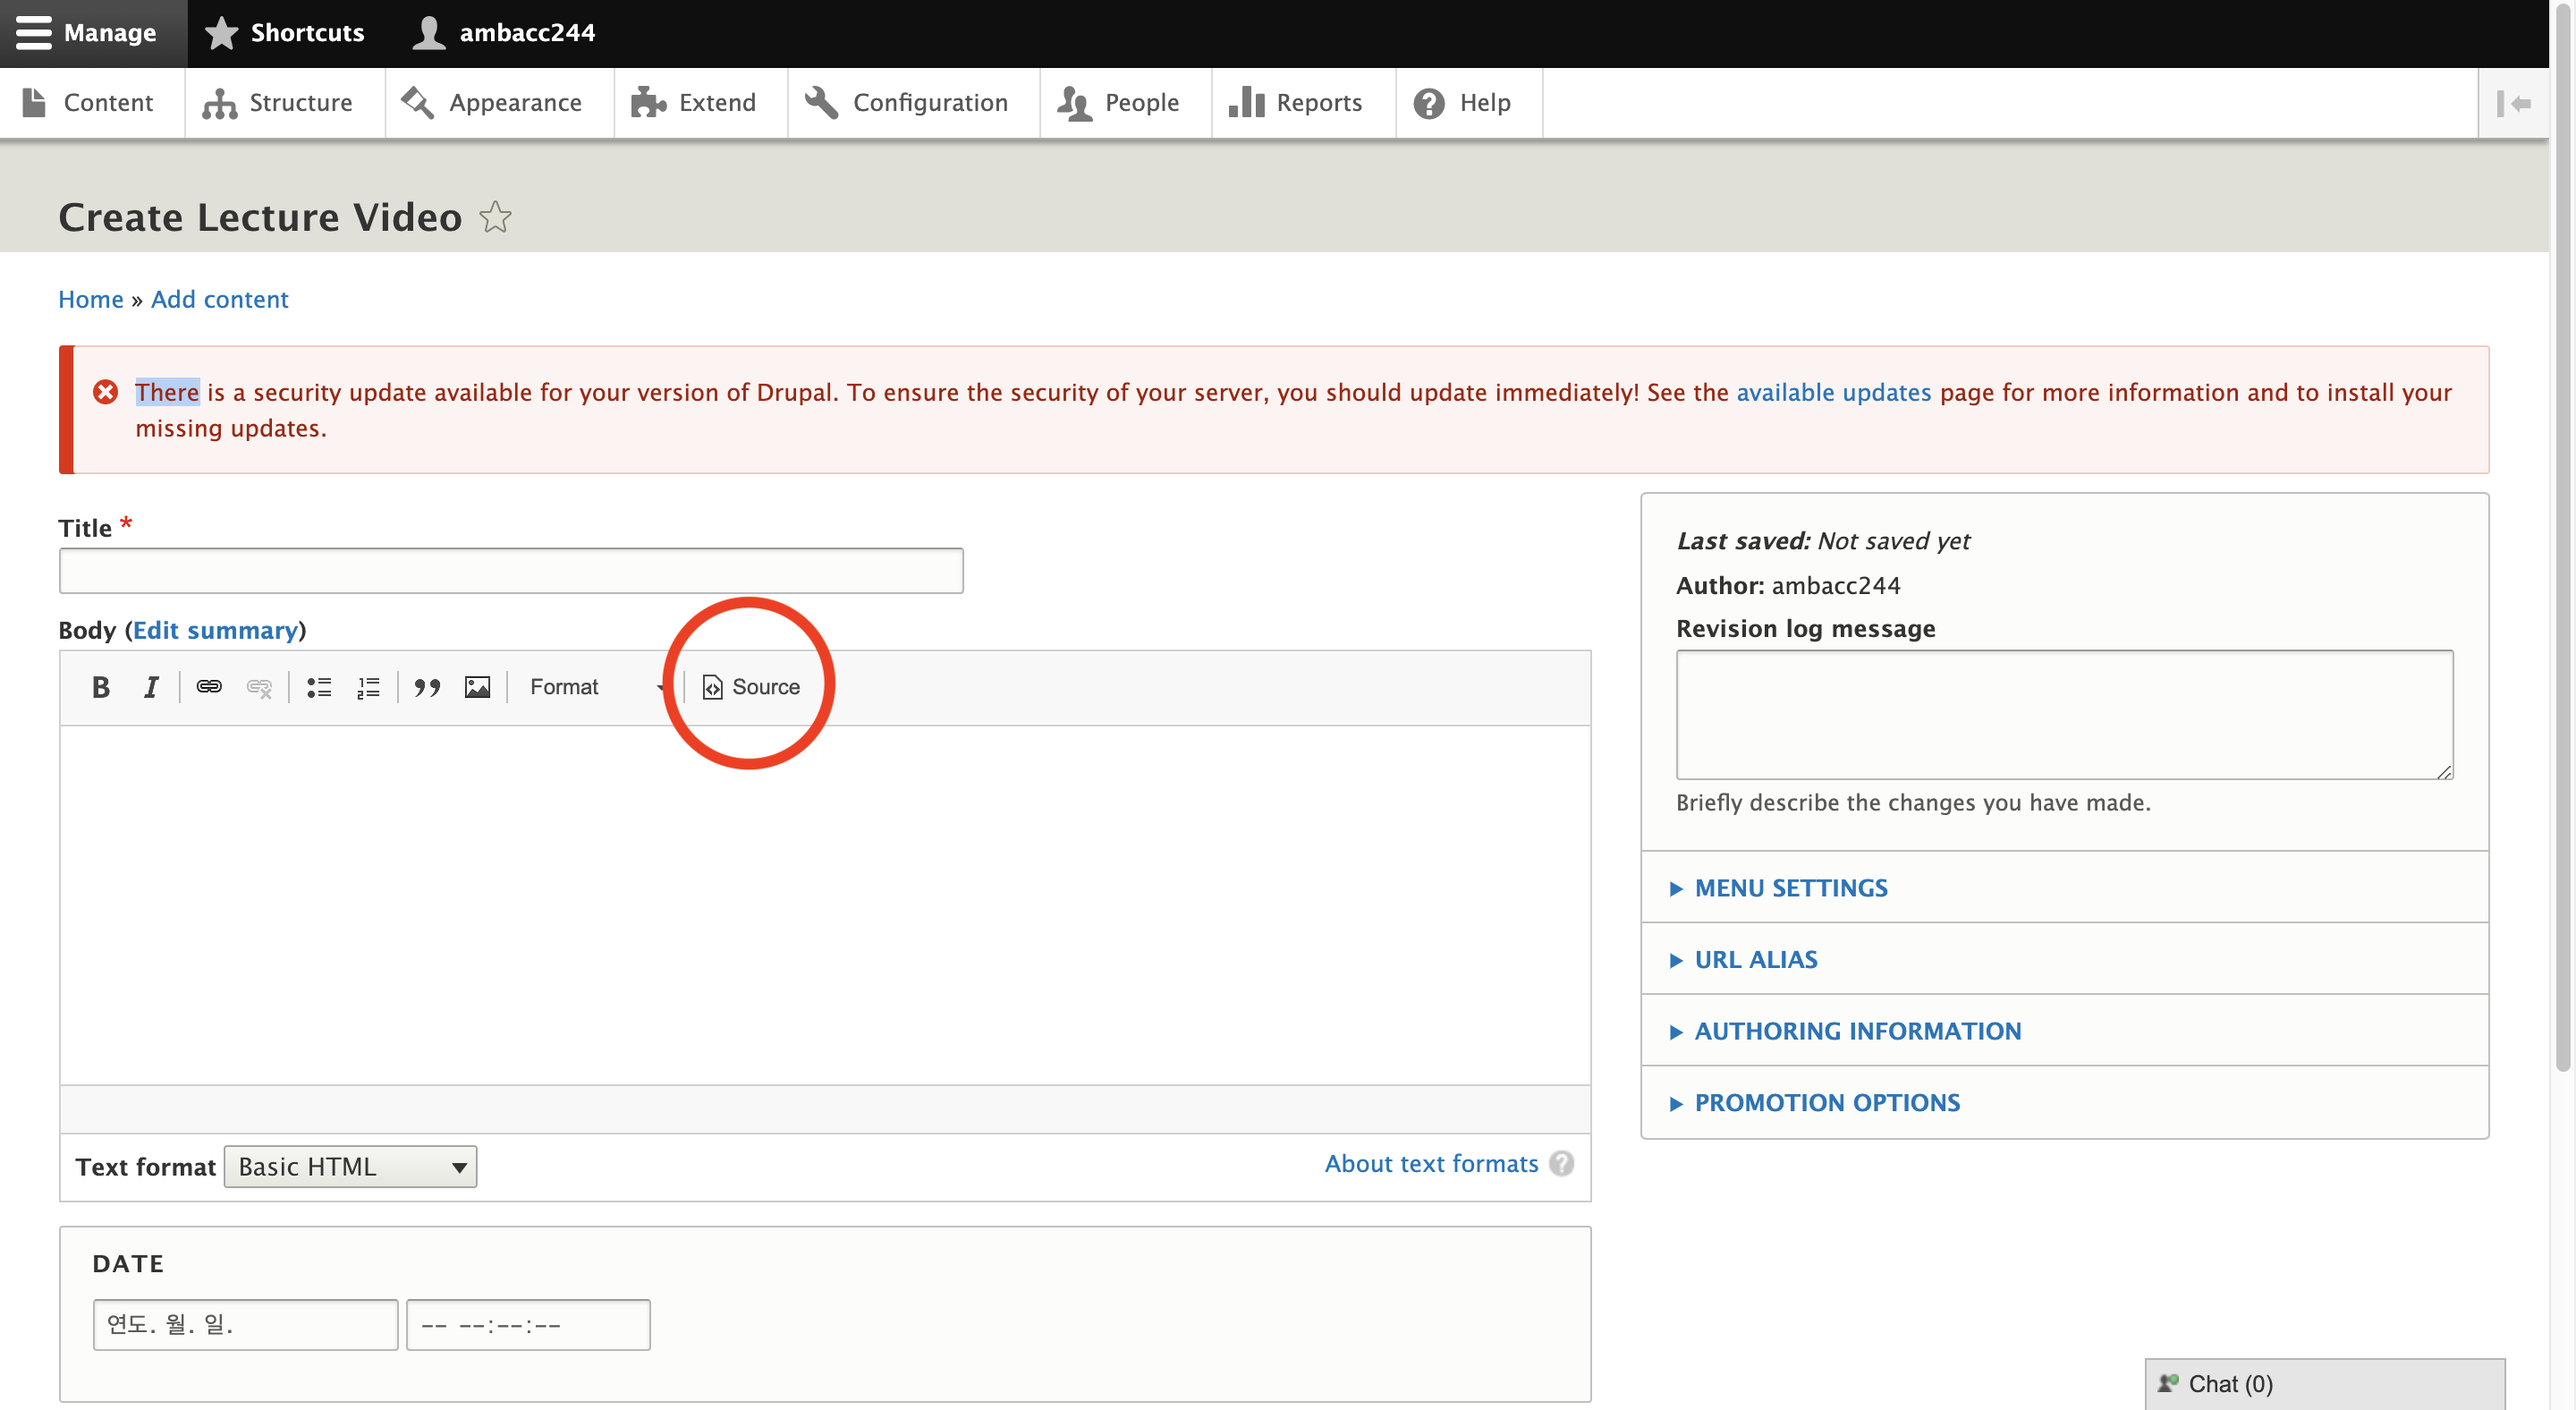
\includegraphics[width=0.7\textwidth]{Project_Document/source.png}
                        \caption{`Source' Button on the Physics Virtual Classroom Website}
                    \end{figure}
            	\item Change code to create and delete whiteboard buttons.
            \end{enumerate}

        \subsubsection{Create new Administrator Account}
            \begin{enumerate}
                \item Click `People’ on the toolbar.
                    \begin{figure}[!ht]
            	        \centering
                        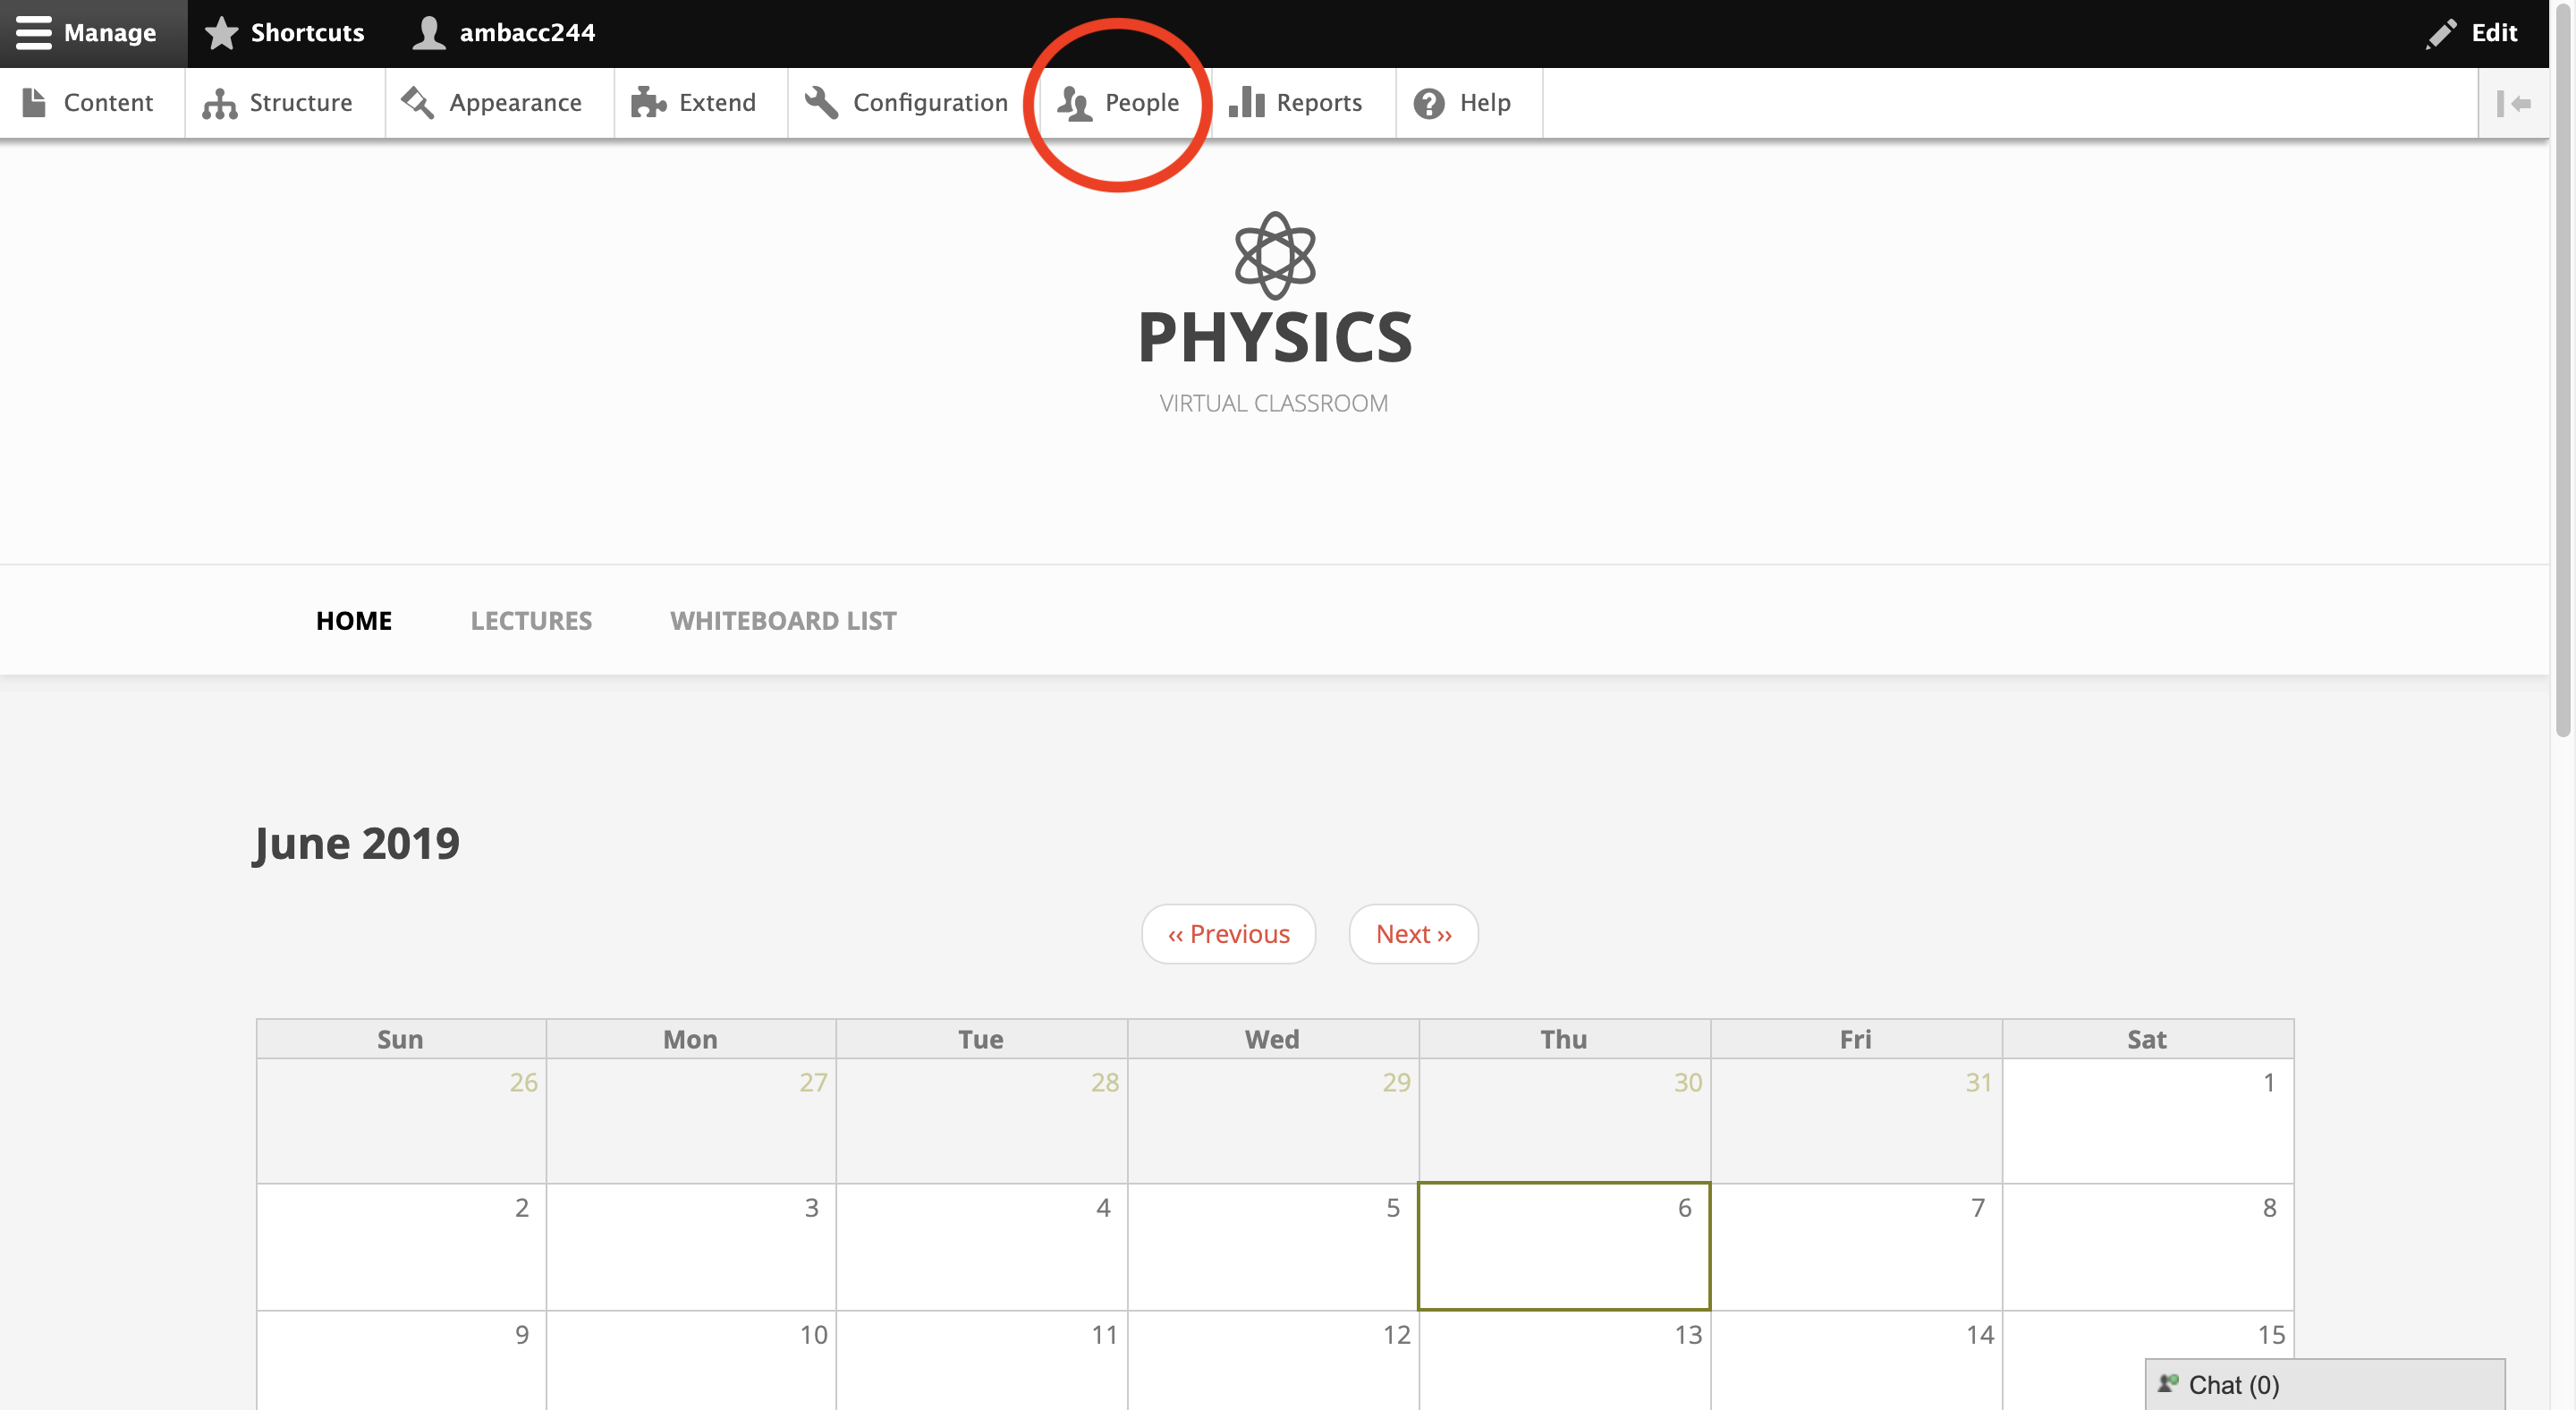
\includegraphics[width=0.7\textwidth]{Project_Document/people.png}
                        \caption{`People' Button on the Physics Virtual Classroom Website}
                    \end{figure}
                \item Click `+Add user'
                \item Need to fill out `Add user' form.
                    \begin{itemize}
                        \item Email address: Optional
                        \item Username: Required
                        \item Password: Required
                        \item Status: Set as  `Active’
                        \item Roles: \textbf{Set as `Administrator'}
                        \item Picture: Optional
                    \end{itemize}
                \item Click `Create new account’
            \end{enumerate}

    \subsection{Back-up Guide}
        If you want to make back-ups of the current website, you need to duplicate the current folder of Drupal and export the current database. Then, follow the above instruction to install or re-install the website. Another easy tool for back-ups may be available as a module. You may want to find it at Drupal's module website.

    \subsection{Additional Information}
        \begin{enumerate}
            \item The website does not require any permission to read any contents on the website. If you want to fix this, you need to download a module that will block anonymous users to read the specific contents of the website.
            \item Drupal encourages users to keep the website up-to-date. Updating the website may cause some problems, so it’s always good to have the latest back-ups.
            \item Currently, the website is run on `http’, not `https’. Some browsers may show a warning message because of the security issue. This can be fixed within the server. You also may want to change some settings of Drupal.

            \item When you upload content, URL of the content may be ugly. It looks like this: drupal.org/node\#\#. So, you may want to change the URL of the content manually. The feature can be found where you can edit the content. (It’s called URL ALIAS) It looks better if you keep adding numbers of what you are posting. For example, /lecture1, /lecture2. There may some module that makes this automatic, but we could not find it.

            \item The whiteboards in the list of whiteboards are currently managed by Eric’s account on AWW. This whiteboard may be removed if the whiteboard hasn’t used for a long time. In case, you may want to create your own account on AWW and make the whiteboards. It will last a very long time (we haven’t checked how long those last).
            \item Drupal can be easily crushed if you make an inappropriate change. So, please test it on your local machine and apply it on the main server.
        \end{enumerate}
\clearpage
\section{Recommended Technical Resources for Learning More}
        We have used the following website the build the whole website:
        \begin{itemize}
            \item https://www.drupal.org/
            \item https://www.awwapp.com/
        \end{itemize}
        \medskip
        People,who have helped or will maintain the website:
                \begin{itemize}
            \item Dr. Kenneth C. Walsh (Professor, client)
            \item Max Moulds (The head programmer of the project)
            \item CoSINe IT Services(They will take a charge of the project after us)
        \end{itemize}

\section{Conclusions and Reflections}
    \subsection{Yeongae Lee}
        The biggest thing that I learned from this project is Drupal. Drupal is software that makes building a website conveniently. It takes time to learn how to use it for the first time, but once you get used to it, it will save a lot of time creating the website. Through this project, I have also learned how the project is going on in real work. This is expected to be useful in the workplace. I think work management did not work well during this project. We aimed to complete the project according to the schedule of the Gantt chart, but we could not actually follow the schedule. As the design of the project continued to change, we could not handle the things we needed to do and gradually delayed. Therefore, we processed most of the works in the last three weeks. In order to complete a project efficiently, works should be divided in detail and managed them on schedule. This project was never easy. Due to the absence of two members, the amount of works is increased. We spent a lot of time to figure exactly goal because of the interruption of conversations with other project groups. If the last team member also left the project, I think it would have been really hard to complete the project by myself. What I felt while doing the project is the importance of conversation among the team members and solid design. I think the difficulties that have been going on in the project are not fulfilling these two points.

    \subsection{Jaehyung You}
        We have learned how to integrate two different APIs into one website during the project.
        We have learned what CMS (Content Management System) is and how to use it. I learned once again that designing a website always takes into account who the targets are. Since we are making a website that targets Physics students, we have to figure out which feature could be helpful to the students. During the project was going, I have known that completing even one project is a very hard achievement. Gathering ideas, designing, and implementing can not be done without a solid teamwork. We had a 4 members at the beginning, and 2 of them were left during the project. It was hard at the time, but it seems to be an opportunity that I can learn more after we overcame it. As a result of this, we have had a more conversation and cooperation with Yeongae on the work. We also learned a lot about project management by adjusting the scale and details of the project. Our original design of the project was a bit different than the current. We have changed it by talking with the client and the head programmer. Therefore, we finally made the something that can be called a ‘project’.  She, Yeongae,and I worked really hard to finish the project on time. If I could do this all over, I would plan the project more wisely. Since we’ve missed some members of the team, our plan was ruined. It made us run out of time. If we had more time, we could add more fun and interesting features. I would like to try different project if there are projects for the students and schools. It makes me really proud. Overall, it was a hard work, but it is totally worth to do it.

\newpage

\begin{thebibliography}{9}

\bibitem{AWW}
AWW App. Online Whiteboard for Realtime Visual Collaboration
\\\texttt{https://awwapp.com/}

\bibitem{AWW APP Price}
AWW App. Pricing
\\\texttt{https://awwapp.com/pricing/}

\bibitem{Chatwing Price}
Chatwing. Pricing
\\\texttt{https://chatwing.com/site/pricing}

\bibitem{fs}
Flask-SocketIO
\\\texttt{https://flask-socketio.readthedocs.io/en/latest/}

\bibitem{Front-end Frameworks}
Ivaylo Gerchev. The 5 Most Popular Front-end Frameworks Compared
\\\texttt{https://www.sitepoint.com/most-popular-frontend-frameworks-compared/}

\bibitem{LiveAgent Price}
LiveAgent. Pricing
\\\texttt{https://www.ladesk.com/pricing/}

\bibitem{Online Whiteboards}
Matt Grech. The 10 Best Online Whiteboards with Realtime Collaboration
\\\texttt{https://getvoip.com/blog/2016/09/14/online-whiteboard-collaboration/}

\bibitem{azure}
Microsoft Azure Cloud Computing Platform \& Services
\\\texttt{https://azure.microsoft.com/en-us/)}

\bibitem{mongo}
MongoDB: Open Source Document Database
\\\texttt{https://www.mongodb.com}

\bibitem{mysql}
MySQL
\\\texttt{https://www.mysql.com/)}

\bibitem{RealTime Board Price}
RealTime Board. Choose your plan
\\\texttt{Retrieved from https://realtimeboard.com/pricing/}

\bibitem{si}
Socket.io
\\\texttt{https://socket.io/}

\bibitem{TW}
Tutorials Point - Online Free Whiteboard
\\\texttt{https://www.tutorialspoint.com/}

\bibitem{ws}
ws - npm
\\\texttt{https://www.npmjs.com/package/ws}

\bibitem{Zite}
Ziteboard | Online Whiteboard with Realtime Collaboration
\\\texttt{https://ziteboard.com/}

\end{thebibliography}

\end{document}
